\documentclass[12pt]{amsart}
\usepackage{researchmacros}
\usepackage{ytableau}
\usepackage{mathtools}
\usepackage{enumitem}
\usepackage{epstopdf}
\epstopdfsetup{outdir=./}
\usepackage[all]{xy}
\usepackage[vcentermath]{youngtab}


\newlist{todolist}{itemize}{2}
\setlist[todolist]{label=$\square$}
\usepackage{pifont}
\newcommand{\cmark}{\ding{51}}%
\newcommand{\xmark}{\ding{55}}%
\newcommand{\done}{\rlap{$\square$}{\raisebox{2pt}{\large\hspace{1pt}\cmark}}%
\hspace{-2.5pt}}



\title{Springer fibers and the Delta Conjecture at $t=0$}
\author{Sean T. Griffin, Jake Levinson, and Alexander Woo}
\date{\today}

\renewcommand{\top}{\mathrm{top}}
\newcommand{\std}{\mathrm{std}}
\newcommand{\conv}{\mathrm{conv}}
\newcommand{\sch}{\mathfrak{S}}
\newcommand{\init}{\mathrm{init}}
\newcommand{\Inv}{\mathrm{Inv}}
\newcommand{\st}{\,|\,}
\newcommand{\vspan}{\mathrm{span}}
\newcommand{\bA}{\mathbb{A}}
\newcommand{\Fl}{\mathrm{Fl}}
\newcommand{\Hilb}{\mathrm{Hilb}}
\newcommand{\Frob}{\mathrm{Frob}}
\newcommand{\la}{\lambda}
\newcommand{\im}{\mathrm{im}}
\newcommand{\SYT}{\mathrm{SYT}}
\newcommand{\sort}{\mathrm{sort}}
\newcommand{\fl}{\mathrm{f\hspace{0.25pt}l}}
\newcommand{\ufl}{\mathrm{ufl}}
\newcommand{\inv}{\mathrm{inv}}
\newcommand{\Hom}{\mathrm{Hom}}
\newcommand{\sh}{\mathrm{sh}}
\newcommand{\bx}{\mathbf{x}}





\newtheorem{question}{Question}




%%%% commenting %%%%
\newcommand{\JL}[1]{{\color{blue} JL: #1}}
\newcommand{\SG}[1]{{\color{red} SG: #1}}
\newcommand{\AW}[1]{{\color{green} AW: #1}}



\usepackage[inline]{showlabels}
\begin{document}
\maketitle

\begin{abstract}
We introduce a family of varieties $Y_{n,\lambda,s}$, \SG{which we call the \emph{$\Delta$-Springer varieties}}, that generalize the type A Springer fibers. We give an explicit presentation of the cohomology ring $H^*(Y_{n,\lambda,s})$ and show that there is a symmetric group action on this ring that generalizes the Springer action on the cohomology of a Springer fiber. The $\lambda=(1^k)$ case of this construction gives a new geometric realization for the expression in the Delta Conjecture when $t=0$. We also prove that the top cohomology groups of these varieties give a generalization of the type A Springer correspondence to the setting of induced Specht modules. Finally, we generalize results of de Concini and Procesi. Precisely, we find a topological space $Y_{n,\lambda}$ whose cohomology ring is isomorphic to the coordinate ring of the scheme of ``rank deficient'' diagonal matrices.
\end{abstract}

\vspace{1cm}

{\color{red} To Do:
\begin{todolist}
\item Subsec 2.1, Background: Schubert cells
\item[\done] Subsec 2.6, Background: $R_{n,\la,s}$
\item Sec 3, Add a full example of affine paving
\item[\done] Sec 5, Rewrite using new notations
\item Sec 7, Define $Y_{n,\la}$, show its cohomology is $R_{n,\la}$, state that this cohomology is iso to the coord ring of the diagonal rank scheme
\item Sec 8, Perhaps add an example of the partial orders on the set of admissible permutations, and the bijection with ordered set partitions in the case of $\lambda = (1^k)$ and $s=k$.
\end{todolist}
}



%%%%%%%%%%%%%%%%%%%%%%%%%%%%
\section{Introduction}\label{sec:Introduction}
%%%%%%%%%%%%%%%%%%%%%%%%%%%%
In this article, we introduce a family of varieties generalizing the Springer fibers. We prove an explicit presentation of their cohomology rings generalizing the one given by Tanisaki for the cohomology ring of a Springer fiber, which coincides with the rings $R_{n,\lambda,s}$ introduced by the first author~\cite{GriffinOSP}. As a special case, our construction gives a new \emph{compact} geometric realization of the  expression in the Delta Conjecture in the case $t=0$. We also prove a version of the Springer correspondence for this family of varieties, showing that their top cohomology groups have the $S_n$-module structure of an induced Specht module. Finally, we generalize work of de Concini and Procesi~\cite{dCP} by introducing a topological space whose cohomology ring coincides with the coordinate ring of the scheme-theoretic intersection of an Eisenbud--Saltman rank variety with diagonal matrices. 




In the seminal work~\cite{Springer-TrigSum,Springer-WeylGrpReps}, T.A. Springer introduced a family of varieties associated to any complete flag variety $G/B$, called Springer fibers, that have remarkable connections to the representation theory of Weyl groups. Springer proved that although the Weyl group does not act on a Springer fiber, it does act nontrivially on the cohomology ring of a Springer fiber. Furthermore, Springer proved that the highest degree nonzero cohomology group of a Springer fiber is (in type A) an irreducible representation of the Weyl group, and every irreducible representation appears this way. This is known as the \emph{Springer correspondence}. We note that the $S_n$-action discussed in this paper differs from Springer's original construction by tensoring with the sign representation.

The graded $S_n$-module type of the cohomology ring of a Springer fiber was discovered by Hotta and Springer~\cite{Hotta-Springer}. Under the Frobenius characteristic map $\Frob$ that associates a symmetric function to each $S_n$-module, the cohomology ring of a Springer fiber is sent to the \emph{modified Hall-Littlewood symmetric function}
\begin{align}
\Frob(H^*(\cB^\lambda;\bQ);q) = \widetilde H_\lambda(x;q^2),
\end{align}
where the $q$ on the left-hand side keeps track of the grading of the cohomology ring. A detailed analysis of this connection has been given by Garsia and Procesi~\cite{Garsia-Procesi}, who were inspired by the explicit quotient ring presentations for $H^*(\cB^\lambda;\bQ)$ discovered by De Concini-Procesi~\cite{dCP} and Tanisaki~\cite{Tanisaki}.

The Delta Conjecture of Haglund--Remmel--Wilson~\cite{HRW} predicts two combinatorial formulas for a particular symmetric function with $q$ and $t$ parameters $\Delta'_{e_{k-1}} e_n(q, t)$ coming from the theory of Macdonald polynomials. The conjecture is known to be true in several special cases, and the \emph{rise} version of the conjecture has recently been proven in full generality~\cite{DM}. Since $\Delta'_{e_{k-1}} e_n$ is conjectured to be Schur-positive, there is much interest in a natural algebraic or geometric construction of a (bigraded) $S_n$-module whose Frobenius characteristic is $\Delta'_{e_{k-1}} e_n$. Haglund--Rhoades--Shimozono~\cite{HRS1} did this in the case $t=0$ by constructing a graded ring $R_{n,k}$ with a suitable $S_n$-action whose graded Frobenius characteristic is $\Delta'_{e_{k-1}} e_n(q, 0)$ (after a minor twist).

Pawlowski and Rhoades~\cite{Pawlowski-Rhoades} gave a parallel geometric interpretation by exhibiting a complex algebraic variety whose cohomology ring is $R_{n,k}$. Since the Hilbert series of $R_{n,k}$ is not symmetric, such a variety must be either non-compact or singular by Poincar\'e Duality. Pawlowski defined the non-compact smooth space of \emph{spanning line arrangements}, $n$-tuples of lines in $\bC^k$ that span $\bC^k$,
\begin{align}
X_{n,k} \coloneqq \{(L_1,\dots, L_n) \in (\bP^{k-1})^n \st L_1+\cdots +L_n = \bC^k\}.
\end{align}
They proved that 
\begin{align}
H^*(X_{n,k}) \cong R_{n,k},
\end{align}
thus giving a connection between the expression in the Delta Conjecture at $t=0$ and geometry. 
Since the Poincar\'e series recording the graded dimensions of the ring $R_{n,k}$ is not symmetric, then by Poincar\'e duality, any complex variety whose cohomology ring is isomorphic to $R_{n,k}$ must either be noncompact or singular. 

In this article, we introduce a compact and singular variety $Y_{n,(1^k),k}$, similar to a Springer fiber, whose cohomology ring is the Haglund--Rhoades--Shimozono ring $R_{n,k}$. Thus, the variety $Y_{n,(1^k),k}$ gives a new geometric realization of the expression in the Delta Conjecture when $t=0$. Furthermore, the family $Y_{n,(1^k),k}$ extends to a family of varieties $Y_{n,\lambda,s}$ generalizing the Springer fibers. This allows us to use techniques from the study of Springer fibers to analyze our varieties. Furthermore, it situates the study of $R_{n,k}$ and $\Delta'_{e_{k-1}}e_n$ in the context of the theory of Springer fibers and geometric representation theory.


As our main result, we prove an explicit presentation of the ring $H^*(Y_{n,\la,s})$ as a quotient of a polynomial ring, generalization Tanisaki's presentation for the cohomology ring of a Springer fiber~\cite{Tanisaki}. This presentation coincides with the graded ring $R_{n,\lambda,s}$ recently introduced by the first author~\cite{GriffinOSP}. 
As a consequence, we see that the cohomology ring of $Y_{n,\lambda,s}$ has a graded $S_n$-module structure generalizing the classical one in the Springer fiber case.

We use results of the first author to prove a generalization of the  Springer correspondence to the setting of induced Specht modules. We show that for $s>\ell(\lambda)$, 
\begin{align}
H^{2d}(Y_{n,\lambda,s};\bQ) \cong \mathrm{Ind}\!\uparrow_{S_k}^{S_n} (S^\lambda),
\end{align}
where $d$ is the dimension of the variety $Y_{n,\lambda,s}$ and $S^\la$ is the irreducible Specht module indexed by $\lambda$. In the special case when $s=\ell(\lambda)$, we show that the top cohomology group is a skew Specht module $S^{\Lambda/(n-k)^{s-1}}$. We also prove that $Y_{n,\lambda,s}$ is equidimensional of complex dimension
\begin{align}
    d = \sum_i \binom{\lambda_i'}{2} + (s-1)(n-k),
\end{align}
and we give a characterization of the irreducible components of $Y_{n,\la,s}$.

Finally, we generalize results of de Concini and Procesi~\cite{dCP}. Let $\mathfrak{gl}_n$ be the Lie algebra of $n\times n$ matrices over $\bQ$. Given $\la\vdash n$, define $O_\lambda\subseteq \mathfrak{gl}_n$ to be the set of $n\times n$ nilpotent matrices over $\bQ$ with Jordan type $\lambda$, and let $\overline{O}_\lambda$ be its closure in $\mathfrak{gl}_n$. Let $\mathfrak{t}\subset \mathfrak{gl}_n$ be the Cartan subalgebra of diagonal matrices. Then de Concini and Procesi proved that
\begin{align}
    H^*(\cB^\la;\bQ) \cong \bQ[\overline{O}_{\la'}\cap \mathfrak{t}],
\end{align}
where the right-hand side is the coordinate ring of the scheme-theoretic intersection of $\overline{O}_{\la'}$ and $\mathfrak{t}$. Given a partition $\lambda$ of size at most $n$, let $\overline{O}_{n,\la}$ be the Eisenbud--Saltman rank variety (defined in Section~\ref{sec:IndVariety}). We define the direct limit space $Y_{n,\la} \coloneqq \varinjlim_s Y_{n,\la,s}$ and prove that there is an isomorphism of graded rings and graded $S_n$-modules
\begin{align}\label{eq:dCPGeneralization}
    H^*(Y_{n,\la};\bQ) \cong \bQ[\overline{O}_{n,\la'}\cap \mathfrak{t}].
\end{align}

In Section~\ref{sec:Background}, we outline preliminary definitions and previous results. In Section~\ref{sec:AffinePaving}, we define the variety $Y_{n,\lambda,s}$ and prove that it has an affine paving, which is a slight modification of Shimomura's paving of a Steinberg variety~\cite{Shimomura}, by intersecting $Y_{n,\lambda,s}$ with Schubert cells. We prove that the cells of this paving have an inductive structure that allows us to compute the rank generating function of the cohomology ring.
In Section~\ref{sec:EmptyPartition}, we analyze the case of $\lambda=\emptyset$ and prove that the variety $Y_{n,\emptyset,s}$ has the same cohomology ring as a product of projective spaces.
In Section~\ref{sec:SpaltensteinAndCohomology}, we show that $Y_{n,\la,s}$ is the image of a projection down from a Spaltenstein variety, and we us this to prove a presentation of the cohomology ring of $Y_{n,\lambda,s}$ as a quotient ring.
In Section~\ref{sec:IrreducibleComponents}, we prove our generalization of the Springer correspondence, and we characterize the irreducible components of $Y_{n,\la,s}$.
In Section~\ref{sec:IndVariety}, we introduce $Y_{n,\la}$ and prove the isomorphism \eqref{eq:dCPGeneralization}.
Finally, in Section~\ref{sec:FutureWork} we list some open problems.






%%%%%%%%%%%%%%%%%%%%%%%%%%%%
\section{Background}\label{sec:Background}
%%%%%%%%%%%%%%%%%%%%%%%%%%%%


\subsection{Flag varieties and Schubert cells}


\SG{To do: Finish this section}

Given a vector space $V$, a \emph{partial flag} is a nested sequence of vector subspaces of $V$,
\begin{align}
    V_\bullet = (V_1\subset V_2\subset\dots\subset V_m).
\end{align}
Given a composition $\alpha = (\alpha_1,\dots, \alpha_m)$ of size at most $\dim(V)$ with $\alpha_i>0$,  define the \emph{partial flag variety} to be the set of partial flags of $V$ such that the dimensions of the successive quotients $V_i/V_{i-1}$ are given by $\alpha$,
\begin{align}
    \Fl_{\alpha}(V) \coloneqq \{V_\bullet = (V_1\subset\dots\subset V_m) \st  \dim(V_i/V_{i-1}) = \alpha_i\text{ for }i\leq m\}.
\end{align}
In the case when $V = \bC^n$ and $\alpha = (1^n)$, we recover the \emph{complete flag variety}, denoted by $\Fl(n) = \Fl_{(1^n)}(\bC^n)$.

\SG{To do: Define Schubert cells and Schubert varieties. State the fact that the PD classes of the Schubert varieties are a basis of cohomology here?}

\SG{Should we switch to indexing partial flag varieties by compositions and include the ambient space in our flag? If so, we should be careful about the Schubert conditions ($NV_i\subseteq V_i$ is different from $NV_i\subseteq V_{i-1}$ in that case)}

\subsection{Chern classes} 

Given a complex vector bundle $E$ on a topological space $X$, the $i$th Chern class of $E$ is a distinguished cohomology class $c_i(E)\in H^{2i}(X)$, where $c_0(E) = 1$. The Chern classes are invariants of the vector bundle, in the sense that if two vector bundles on $X$ are isomorphic, then their Chern classes agree.  

The sum of the Chern classes of a vector bundle $c(E) \coloneqq 1+c_1(E) + c_2(E) +\cdots$ is called the {\bf total Chern class} of $E$. It has the following useful properties.
\begin{itemize}
    \item Naturality: For any continuous map $f : X \to Y$ and any complex vector bundle $E$ on $Y$, then $f^*(c(E)) = c(f^*(E))$, where the first $f^*$ is the map on cohomology and $f^*(E)$ is the pullback of $E$.
    \item Additivity: Given a short exact sequence of vector bundles $0\to E'\to E\to E''\to 0$ on $X$, we have
    \begin{align}
        c(E) = c(E')c(E''),
    \end{align}
    where multiplication is via the cup product on cohomology.
    \item Vanishing: If $r$ is the rank of $E$ as a complex vector bundle, then $c_i(E) = 0$ for all $i>r$.
    \item Triviality: If $E \cong \bC^r \times X$, a trivial vector bundle, then $c(E) = 1$.
\end{itemize}

In the case of $X = \Fl(\bC^n)$, for each $j$ there is the tautological vector bundle $\widetilde V_j$ whose fiber over $V_\bullet = (V_1,\dots, V_n)$ is the vector space $V_{j}$. Borel~\cite{Borel} proved that the classes $c_1(\widetilde V_j/\widetilde V_{j-1})$ generate the cohomology ring $H^*(\Fl(\bC^n))$ as a graded algebra. Moreover, there is an isomorphism of graded algebras,
\begin{align}\label{eq:BorelTheorem}
    H^*(\Fl(\bC^n)) \cong \frac{\bZ[x_1,\dots, x_n]}{\langle e_1(x_1,\dots, x_n),\dots, e_n(x_1,\dots, x_n)\rangle}
\end{align}
identifying $-c_1(\widetilde V_j/\widetilde V_{j-1})$ with $x_j$, where each variable $x_j$ is considered to be degree $2$.
The quotient ring on the right-hand side of \eqref{eq:BorelTheorem} is also known as the \emph{coinvariant ring}.





\subsection{Affine paving}

An affine paving is another tool that we will use for working with cohomology. Given a complex algebraic variety $X$, an {\bf affine paving} of $X$ is a sequence of closed subvarieties
\begin{align}
    X_0 \subseteq X_1\subseteq \cdots \subseteq X_m = X
\end{align}
of $X$ such that $X_i\setminus X_{i-1} \cong \bigsqcup_j A_{i,j}$ for locally closed subspaces $A_{i,j}$ such that for all $i,j$, $A_{i,j}\cong \bC^k$ for some $k$. The affine spaces $A_{i,j}$ are called the {\bf cells} of the affine paving.

An affine paving allows us to compute the ranks of the cohomology groups of $X$ with compact support. When $X$ is compact in the analytic topology, cohomology with compact support is the same as cohomology, so an affine paving gives us a way of computing the ranks of the cohomology groups.

\begin{lemma}\label{lem:OddCohVanishes}
Suppose $X$ is a smooth or compact complex algebraic variety that has an affine paving. If $X_i\setminus X_{i-1} = \bigsqcup_{i,j} A_{i,j}$ is the decomposition of $X$ into affine spaces, then
\begin{align}
    H^{2k}_c(X) &\cong \bZ^{\#\{(i,j) \st \dim_\bC(A_{i,j}) = k\}}\\
    H^{2k+1}_c(X) & = 0,
\end{align}
for all $k\geq 0$.
\end{lemma}

Under certain conditions, affine pavings can also be used to prove that the map on cohomology corresponding to a continuous map is injective or surjective.
%
\begin{lemma}\label{lem:PavingSurj}
Suppose $X$ is a smooth compact complex algebraic variety and $Y\subseteq X$ is a closed subvariety of $X$. If $Y$ and $X\setminus Y$ have affine pavings, then the map on cohomology
\begin{align}
H^*(X)\to H^*(Y)
\end{align}
induced by the inclusion $Y\subseteq X$
is surjective.
\end{lemma}
\begin{proof}
By Lemma~\ref{lem:OddCohVanishes}, all odd cohomology groups of $X$ and $Y$ and all odd cohomology groups with compact support of $X\setminus Y$ are zero. By the long exact sequence for compactly supported cohomology associated to the diagram $Y\hookrightarrow X\hookleftarrow X\setminus Y$, we have short exact sequences
\begin{align}\label{eq:SESCoh}
0 \to H^{2i}_c(X\setminus Y) \to H^{2i}(X) \to H^{2i}(Y)\to 0
\end{align}
for all $i$.
The surjectivity of the map on cohomology then follows from \eqref{eq:SESCoh}.
\end{proof}

\begin{lemma}\label{lem:InjectiveCoh}
Suppose $f: X\to Y$ is a surjective continuous map between compact complex algebraic varieties. Suppose that $Y$ has an affine paving such that for each cell $A_{i,j}$,
\begin{align}
    f^{-1}(A_{i,j}) \cong Z_{i,j}\times A_{i,j}
\end{align}
for some nonempty compact complex algebraic variety $Z_{i,j}$ with an affine paving. Then the map on cohomology
\begin{align}
    H^*(Y)\to H^*(X)
\end{align}
is injective.
\end{lemma}

\begin{proof}
\SG{The proof is currently not correct as written, because the homology is generated by the \emph{closure} of the cells :/ Need to fix!!} Since $Y$ has an affine paving, and $f^{-1}(A_{i,j})\cong Z_{i,j} \times A_{i,j}$, it can be seen that $X$ has an affine paving with cells $C\times A_{i,j}$, where $C$ runs over all cells of $Z_{i,j}$. 
 Therefore, $H_*(X)$ is freely generated by the fundamental classes $[C\times A_{i,j}]$. 

Since $Z_{i,j}$ is compact, there is a cell of $Z_{i,j}$ consisting of a single point, $C = \{\text{pt}\}$. Letting $f_* : H_*(X)\to H_*(Y)$ be the map on homology induced by $f$, we have
\begin{align}
f_*([\{\text{pt}\}\times A_{i,j}]) = [A_{i,j}],
\end{align}
hence $f_*$ is surjective. 
By the Universal Coefficient Theorem, the map $f^*$ is the dual of $f_*$, which is thus injective.
\end{proof}

\subsection{Springer fibers}

Given a partition $\lambda$ of $n$, let $N_\lambda$ be a $n\times n$ nilpotent matrix whose Jordan block sizes are recorded by $\lambda$. The {\bf Springer fiber} associated to $\lambda$ is
\begin{align}
    \cB^\lambda \coloneqq \{V_\bullet \in \Fl(n) \st N_\lambda V_i\subseteq V_i \text{ for all } i\leq n\}.
\end{align}
Springer proved that although $S_n$ does not act on $\cB^\lambda$, it does act on the cohomology ring of $\cB^\lambda$. We note that in this article, the action on the cohomology ring we consider differs from the one originally constructed by Springer by tensoring with the sign representation.

A remarkable property of this action is that it gives a geometric construction of the irreducible Specht modules. Indeed, the dimension of $\cB^\lambda$ as a complex variety is 
\begin{align}
    n(\lambda) \coloneqq \sum_i \binom{\lambda_i'}{2},
\end{align}
and the top nonzero cohomology group of $\cB^\lambda$ as an $S_n$-module is
\begin{align}
    H^{2n(\lambda)}(\cB^\lambda;\bQ) \cong S^\lambda.
\end{align}
Therefore, in Lie type A there is a bijection, known as the \emph{Springer correspondence}, between Springer fibers and the irreducible $S_n$-modules, up to isomorphism. 

Hotta and Springer~\cite{Hotta-Springer} proved that the map on cohomology induced by the inclusion $\cB^\lambda \subseteq \Fl(n)$,
\begin{align}
    H^*(\Fl(n)) \to H^*(\cB^\lambda),
\end{align}
is surjective and $S_n$-equivariant. Hence, by surjectivity the cohomology ring $H^*(\cB^\lambda)$ is generated by the cohomology classes $c_1(\widetilde V_i/\widetilde V_{i-1})$. Here, we are abusing notation and writing $\widetilde V_i$ for the restriction of this vector bundle to $\cB^\lambda$. 

There is an explicit presentation of $H^*(\cB^\lambda)$ as a quotient ring extending Borel's theorem~\cite{dCP,Tanisaki}. For all $i\leq n$, let $p_i(\lambda) = \la'_n + \la'_{n-1} +\cdots + \la'_{n-i+1}$, where $\la'_i = 0$ for all $i>\la_1$. Given $S\subseteq \{x_1,\dots, x_n\}$, define $e_d(S)$ to be the sum of all square-free products of variables in $S$ of degree $d$. Define the following ideal and quotient ring,
\begin{align}
    I_\lambda &\coloneqq \langle e_d(S) \st d > |S| - p_{|S|}(\lambda)\rangle,\\
    R_\lambda &\coloneqq \bQ[x_1,\dots, x_n]/I_\lambda.
\end{align}
Here, and throughout the paper, we consider $R_\lambda$ to be a graded ring where each variable $x_j$ is in degree $2$. Tanisaki proved that there is an isomorphism of graded rings
\begin{align}
    H^*(\cB^\lambda;\bQ) \cong R_\lambda
\end{align}
given by identifying the cohomology class $-c_1(\widetilde V_j/\widetilde V_{j-1})$ with the variable $x_j$.

For example, when $\lambda = (2,1)$, then $p_{1}(\lambda) = 0$, $p_2(\lambda) = 1$, and $p_3(\lambda) = 3$. Therefore, $I_\lambda$ is generated by $e_d(S)$ where $3\geq d>0$ and $|S|=3$, or $2\geq d>1$ and $|S| = 2$, so 
\begin{align}
I_{(2,1)} &= \langle e_1(x_1,x_2,x_3), e_2(x_1,x_2,x_3), e_3(x_1,x_2,x_3), e_2(x_1,x_2), e_2(x_1,x_3), e_2(x_2,x_3)\rangle\\
&= \langle x_1+x_2+x_3,\, x_1x_2+x_1x_3+x_2x_3,\, x_1x_2x_3,\, x_1x_2,\, x_1x_3,\, x_2x_3\rangle\\
&= \langle x_1+x_2+x_3,\, x_1x_2,\, x_1x_3,\, x_2x_3\rangle,
\end{align}
and $H^*(\cB^{(2,1)})\cong R_{(2,1)} = \bZ[x_1,x_2,x_3]/I_{(2,1)}$.


\subsection{Symmetric functions and the Delta Conjecture}

The representation theory of the group $S_n$ is closely related to the theory of symmetric functions.
A {\bf symmetric function} is a formal power series in the infinite variable set $\bx = \{x_1,x_2,\dots \}$ that is invariant under any permutation of the variables.
For $\la\vdash n$, let $e_\la(\bx)$ and $s_\la(\bx)$ denote the \emph{elementary symmetric functions} and \emph{Schur symmetric functions}, which form bases of the ring of symmetric functions. 

The Frobenius characteristic map gives a connection between symmetric functions and representations of $S_n$, which we define next. Given $\la\vdash n$, let $S^\la$ be the irreducible $S_n$-module indexed by $\la$, also known as a \emph{Specht module}. Given a finite-dimensional vector space $V$ over $\bQ$ which has the structure of a $S_n$-module, it decomposes as a direct sum of Specht modules
\begin{align}
V\cong \bigoplus_{\la\vdash n}(S^\la)^{c_\la}
\end{align}
for some nonnegative integers $c_\la$. The \emph{Frobenius characteristic} of $V$ is defined to be the symmetric function
\begin{align}
\Frob(V) = \sum_{\la\vdash n} c_\la s_\la(\bx).
\end{align}
Given a graded $S_n$-module $V = \bigoplus_{i = 0}^m V_i$ with finite-dimensional direct summands $V_i$, the \emph{graded Frobenius characteristic} of $V$ is
\begin{align}
\Frob(V;q) = \sum_{i=0}^m \Frob(V_i)q^i.
\end{align}


One well-known family of symmetric functions is the \emph{Macdonald symmetric functions} $\widetilde H_\lambda(\bx;q,t)$. In Mark Haiman's groundbreaking work~\cite{Haiman01,Haiman02}, he proved that $\widetilde H_\lambda(\bx;q,t)$ is the Frobenius character of the bigraded \emph{Garsia-Haiman module}~\cite{Garsia-Haiman}. 
One piece of Haiman's analysis uses linear operators $\Delta'_f$ on the space of symmetric functions~\cite{BGHT} whose eigenbasis is the set of Macdonald functions $\widetilde H_\lambda(\bx;q,t)$. 

Some major open problems following Haiman's work involve finding combinatorial and geometric interpretations for evaluations of this operator when $f$ is a complete elementary symmetric function.
One such problem, called the Delta Conjecture~\cite{HRW}, predicts two combinatorial formulas for the $q,t$ symmetric function $\Delta'_{e_{k}}e_n(q,t)$
in terms of combinatorial statistics on \emph{parking functions}. 
The Delta Conjecture has recently been proven by D'Adderio--Mellit~\cite{DM} and Blasiak--Haiman--Morse--Pun--Seelinger~\cite{BHMPS}.

There has been an ongoing search for algebraic and geometric interpretations of the expression $\Delta_{e_{k}}e_n(q,t)$ in the Delta Conjecture. Haglund, Rhoades, and Shimozono~\cite{HRS1} found an algebraic interpretation when $t=0$. Precisely, they defined the following ring $R_{n,k}$ depending on two positive integers $k\leq n$,
\begin{align}
    R_{n,k} = \frac{\bZ[x_1,\dots, x_n]}{\langle x_1^k,\dots, x_n^k,e_n,e_{n-1},\dots, e_{n-k+1}\rangle}.
\end{align}
When $k=n$, it can be checked that $R_{n,n}$ is equal to the usual coinvariant ring~\eqref{eq:BorelTheorem}.
They proved that the graded Frobenius characteristic of $R_{n,k}$ is $\Delta'_{e_{k-1}}e_n(q,0)$ at $t=0$, up to a minor twist:
\begin{align}\label{eq:DeltaTZero}
\mathrm{Frob}(R_{n,k};q) = \omega\circ \mathrm{rev}_q (\Delta'_{e_{k-1}}e_n(q,0)),
\end{align}
where $\omega$ and $\mathrm{rev}_q$ are simple idempotent operators on symmetric functions. Pawlowski and Rhoades then found a parallel geometric construction for $R_{n,k}$ as the cohomology ring of a space of spanning line arrangements~\cite{Pawlowski-Rhoades}.
An algebraic interpretation for the $q,t$ symmetric function $\Delta_{e_{k-1}}e_n$ has been conjectured by Zabrocki~\cite{Zabrocki} in terms of the bigraded super-diagonal coinvariant ring.




\subsection{The rings $R_{n,k}$ and $R_{n,\lambda,s}$}

We recall the definition and properties of the ring $R_{n,\la,s}$ introduced by the first author in \cite{GriffinOSP}, which simultaneously generalizes the cohomology ring of a Springer fiber $H^*(\cB^\lambda)$ and the Haglund--Rhoades--Shimozono ring $R_{n,k}$. 

Fix $k\leq n$, a partition $\la\vdash k$, and $s\geq \ell(\la)$.  Let $p^n_m(\la) = \la'_n +\cdots + \la'_{n-m+1}$, where $\la'_i= 0$ for all $i> \la_1$. The ideal $I_{n,\la,s}$ and ring $R_{n,\la,s}$ are defined as follows,
\begin{align}
I_{n,\la,s} &= \langle x_1^s,\dots, x_n^s\rangle + \langle e_d(S) \st S\subseteq \{x_1,\dots, x_n\}, \, d > |S| - p^n_{|S|}(\la)\rangle,\\
R_{n,\la,s} &= \bZ[x_1,\dots, x_n]/I_{n,\la,s}.
\end{align}
It can be checked that
\begin{itemize}
    \item When $n=k$, then $I_{n,\la,s} = I_{\lambda}$ for any $s$, thus $R_{n,\la,s} = R_\la$ in this case.
    \item When $\la = (1^k)$ and $s=k$, then $I_{n,(1^k),k} = I_{n,k}$, thus $R_{n,(1^k),k} = R_{n,k}$.
\end{itemize}

For a further example, let $n=4$, $\lambda = (2,1)$, and $s=2$. Then $I_{4,(2,1),2}$ is generated by $x_i^2$ for $i=1,2,3,4$ and the polynomials 
$e_d(S)$ for $S\subseteq \{x_1,\dots, x_4\}$ such that
\begin{equation*}
\begin{aligned}
	d &= 2 \text{ and }|S| = 4,\\
	d &= 4\text{ and }|S| = 4,\\
\end{aligned}
\qquad
\begin{aligned}
	d &= 3\text{ and }|S| = 4,\\
	d &= 3\text{ and }|S| = 3.
\end{aligned}
\end{equation*}
We have
\begin{align*}
    I_{4,(2,1),2} &= \langle x_1^2,x_2^2,x_3^2,x_4^2,e_2,e_3,e_4,e_3(x_1,x_2,x_3),e_3(x_1,x_2,x_4),e_3(x_1,x_3,x_4),e_3(x_2,x_3,x_4)\rangle,\\
    &= \langle x_1^2,\, x_2^2,\, x_3^2,\, x_4^2,\, x_1x_2+x_1x_3+x_1x_4+x_2x_3+x_2x_4+x_3x_4,\\
    &\qquad x_1x_2x_3+x_1x_2x_4+x_1x_3x_4+x_2x_3x_4,\\ 
    &\qquad x_1x_2x_3x_4,\, x_1x_2x_3,\, x_1x_2x_4,\, x_1x_3x_4,\, x_2x_3x_4\rangle,
\end{align*}
and $R_{4,(2,1),2} = \bZ[x_1,x_2,x_3,x_4]/I_{4,(2,1),2}$. 

Let $I_{n,\lambda,s}^\bQ$ be the ideal in $\bQ[x_1,\dots,x_n]$ given by the same generators as $I_{n,\lambda,s}$, and let $R_{n,\la,s}^\bQ = \bQ[x_1,\dots, x_n]/I_{n,\lambda,s}^\bQ$. 
The first author has proven a basis of $R_{n,\la,s}^\bQ$ generalizing the \emph{Artin basis} of the coinvariant ring. Define $\cA_{1,\emptyset,s} = \{1,x_1,\dots, x_1^{s-1}\}$ and $\cA_{1,(1),s} = \{1\}$. Let the set $\cA_{n,\la,s}$ be defined recursively as follows,
\begin{align}
    \cA_{n,\la,s} \coloneqq \bigsqcup_{i=1}^{\ell(\la)} x_n^{i-1} \cA_{n-1,\la^{(i)},s} \sqcup \bigsqcup_{i=\ell(\la)+1}^s x_n^{i-1} \cA_{n-1,\la,s},
\end{align}
where for $1\leq i \leq \ell(\la)$, $\la^{(i)}$ is the partition obtained by sorting the parts of \[(\la_1,\dots, \la_{i-1},\la_i-1,\la_{i+1},\dots, \la_{\ell(\la)})\]
and deleting a trailing zero if necessary.
Then $\cA_{n,\la,s}$ is a $\bQ$-basis of $R_{n,\la,s}^\bQ$~\cite[Theorem 3.18]{GriffinOSP}.

\SG{Should we move the following lemmata into the body of the paper? They are straightforward from the results in my thesis.}

\begin{lemma}\label{lem:FreeZMod}
The set $\cA_{n,\la,s}$ represents a $\bZ$-basis of $R_{n,\la,s}$.
\end{lemma}
\begin{proof}
The proof of Lemma 3.14 in \cite{GriffinOSP} also proves that $\cA_{n,\la,s}$ is a $\bZ$-spanning set of $R_{n,\la,s}$. Since $\cA_{n,\la,s}$ represents a $\bQ$-linearly independent subset of $R_{n,\la,s}^\bQ$, then it also represents a $\bZ$-linearly independent subset of $R_{n,\la,s}$.
\end{proof}

Given $V = \bigoplus_{i\geq 0} V_i$ a graded free $\bZ$-module with graded pieces $V_i$ of finite rank $\mathrm{rk}(V_i)$, let the \emph{Hilbert--Poincar\'e series} of the module $V$ be 
\begin{align}
    \Hilb(V;q) \coloneqq \sum_{i\geq 0} \mathrm{rk}(V_i)q^i.
\end{align}
By Lemma~\ref{lem:FreeZMod}, $R_{n,\la,s}$ is a free $\bZ$-module. Under our convention that $x_i$ has degree $2$ for all $i$, we have the following recursive formula for the Hilbert series, which follows immediately by Lemma~\ref{lem:FreeZMod}.
\begin{lemma}\label{lem:RHilbRecursion}
We have
\begin{align}
    \Hilb(R_{n,\la,s};q) = \sum_{i=1}^{\ell(\la)} q^{2(i-1)} \Hilb(R_{n-1,\la^{(i)},s};q) + \sum_{i=\ell(\la)+1}^s q^{2(i-1)} \Hilb(R_{n-1,\la,s};q).
\end{align}
\end{lemma}

Since the set of generators of the homogeneous ideal $I_{n,\la,s}$ is closed under the action of $S_n$ permuting variables, $R_{n,\la,s}$ inherits the structure of a graded $S_n$-module. In order to prove our generalization of the Springer correspondence, we make use of a formula for the graded Frobenius characteristic of $R_{n,\la,s}$ proven in~\cite{GriffinOSP}. We state the formula and define the associated combinatorial objects in Section~\ref{sec:IrreducibleComponents} where we need it.




%%%%%%%%%%%%%%%%%%%%%%%%%%%%
\section{Definition of $Y_{n,\lambda,s}$ and an affine paving}\label{sec:AffinePaving}
%%%%%%%%%%%%%%%%%%%%%%%%%%%%

\AW{We should say this is an analogue of the Tymoczko and Precup results for Hessenberg varieties and that we're using a similar approach.}

In this section, we define a family of varieties $Y_{n,\lambda,s}$ that generalize the Springer fibers. We construct an affine paving of $Y_{n,\lambda,s}$ by intersecting it with Schubert cells. The affine paving presented here is a slight modification of the affine pavings given by Fresse, Precup--Tymoczko, and Shimomura for Steinberg varieties~\cite{Fresse,Precup-Tymoczko-Parabolic,Shimomura}. We show that this affine paving has an inductive structure that allows us to show $H^*(Y_{n,\lambda,s})$ and $R_{n,\lambda,s}$ have the same Hilbert--Poincar\'e series.

Let $k\leq n$, where $k$ is a nonnegative integer and $n$ is a positive integer, let $\la\vdash k$, and let $s\geq \ell(\la)$. Define $\Lambda \coloneqq \Lambda(n,\lambda,s) \coloneqq (n-k+\lambda_1,\ldots,n-k+\lambda_s)$ and $K\coloneqq |\Lambda|=s(n-k)+k$. We define a variety $Y_{n,\la,s}$, which is our main object of study.
\begin{definition}
Let $N_\Lambda$ be a nilpotent matrix of Jordan type $\Lambda$. Define
\begin{align}
    Y_{n,\la,s}\coloneqq \{V_\bullet \in \Fl_{(1^n)}(\bC^K)\st N_\Lambda V_i\subseteq V_i\text{ for }i\leq n,\text{ and }\im(N_\Lambda^{n-k})\subseteq V_n\},
\end{align}
where $\im(N_\Lambda^{n-k})$ is the image of the linear map $N_\Lambda^{n-k}: \bC^K\to \bC^K$.
\end{definition}

\SG{How about the \emph{$\Delta$-Springer variety}??}

\begin{remark}
Since $N_\Lambda$ is nilpotent, it can be checked that the set of conditions $N_\Lambda V_i\subseteq V_i$ for $i\leq n$ on a partial flag $V_\bullet\in \Fl_{(1^n)}(\bC^K)$ is equivalent to the set of conditions $N_\Lambda V_i\subseteq V_{i-1}$ for $i\leq n$, where $V_0\coloneqq 0$. Therefore, the variety $Y_{n,\la,s}$ can alternatively be defined as
\begin{align}
    Y_{n,\la,s} = \{V_\bullet \in \Fl_{(1^n)}(\bC^K) \st N_\Lambda V_i\subseteq V_{i-1} \text{ for }i\leq n,\text{ and }\im(N_\Lambda^{n-k})\subseteq V_n\}.
\end{align}
We use these two definitions interchangeably throughout the paper.
\end{remark}
It can be checked that the isomorphism type of $Y_{n,\la,s}$, both as a variety and as a topological space, depends only on $\Lambda$ and not on the choice of $N_\Lambda$. It will be convenient to specify particular choices for $N_\Lambda$, which we do next. 

We denote by $[\Lambda]$ the Young diagram of $\Lambda$, following the English convention, considered as the set
$$[\Lambda]=\{(i,j)\mid 1\leq i\leq \ell(\Lambda), 1\leq j\leq \Lambda_i\}.$$
The cells in column $n-k+1$ and to the right form a copy of the Young diagram of $\lambda$, which we denote by $[\lambda]$. 
We think of a filling of the Young diagram as a function $T:[\Lambda]\rightarrow \mathbb{Z}_{>0}$.
We say that a cell of $[\Lambda]$ or a label of $T$ is on the \textbf{right edge} if it is right most in its row.
See Figure~\ref{fig:Lambda} for an illustration of $[\Lambda]$ and $[\lambda]$, where the cells in the right edge of $[\Lambda]$ are shaded. 
%Given a label $a=T(i,j)$ of $T$ that is not on the right edge, define $s_T(a) \coloneqq T(i,j+1)$, the label immediately to the right of $a$.

\begin{figure}
    \centering
    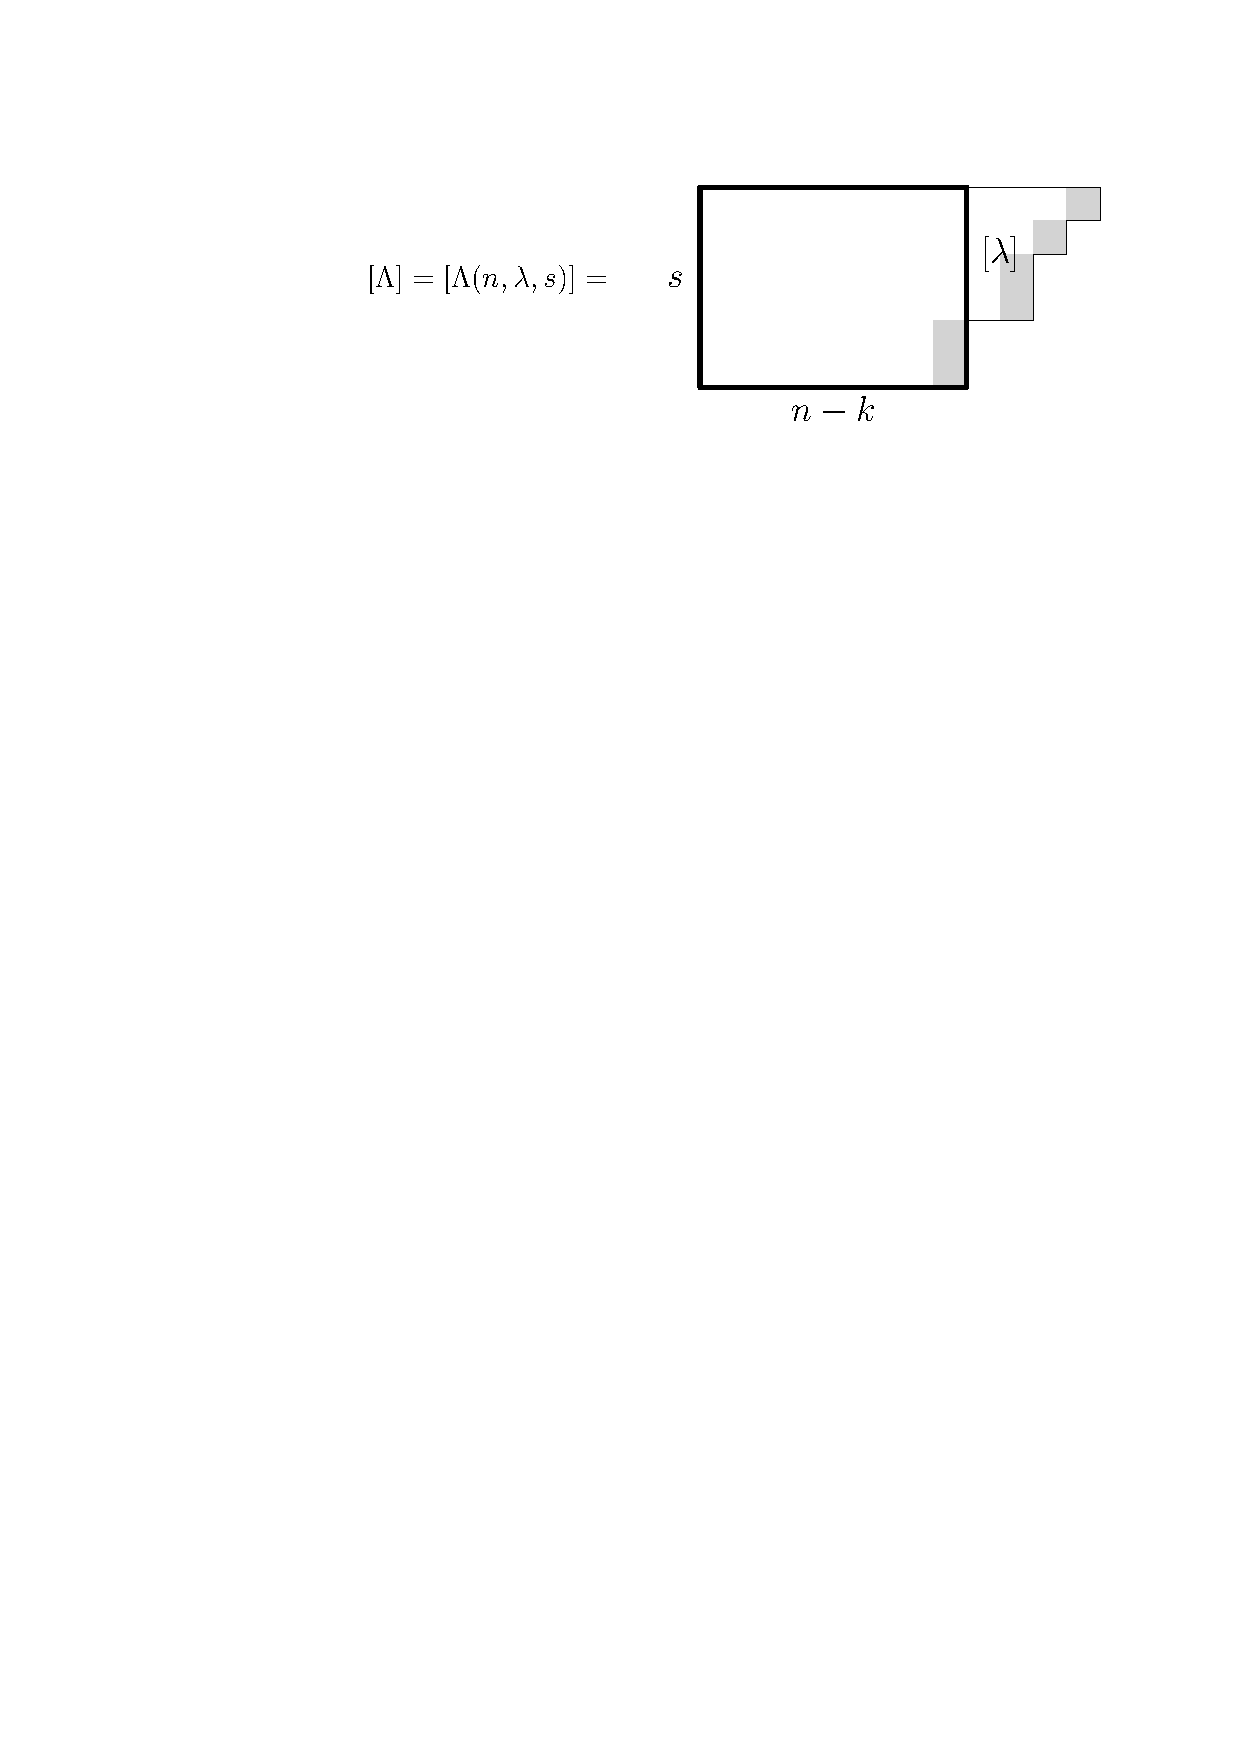
\includegraphics[width=0.7\textwidth]{Figures/LambdaExMain.pdf}
    \caption{The Young diagram $[\Lambda]$, which has a copy of $[\lambda]$ in the upper right corner, highlighted in bold. The cells in the right edge of $[\Lambda]$ are shaded.
    %The maximal cells correspond to flags inducing a particular Jordan type on the nilpotent operator $N$.
    }
    \label{fig:Lambda}
\end{figure}

For any filling $T$ of $[\Lambda]$ satisfying the following conditions,
\begin{enumerate}
\item[(S1)] $T$ is a bijection between $[\Lambda]$ and $\{1,2,\dots, K\}$,
\item[(S2)] $T(i,j)\leq k$ for all $(i,j)\in [\lambda]$,
\end{enumerate}
we define a variety $Y_{T}$, as follows.
Fix an ordered basis $f_1,\ldots,f_K\in \mathbb{C}^K$, let $F_i=\vspan\{f_1,\ldots,f_i\}$ for all $i$ with $1\leq i\leq K$, and  define $N_T$ to be the nilpotent endomorphism
where $N_T(f_{T(i,\Lambda_i)}) = 0$ for $i\leq s$, and  $N_T(f_{T(i,j)})=f_{T(i,j+1)}$ for $i\leq s$ and $j<\Lambda_i$.  Note that $N_T$ has Jordan type
$\Lambda$ by construction.  
Define
\begin{align}
    Y_T \coloneqq Y_{n,\lambda,s,T}\coloneqq \{V_\bullet\in\Fl_{(1^n)}(\mathbb{C}^K) \mid N_TV_i\subseteq V_i\text{ for all } i\text{, and } F_k\subseteq V_n\},
\end{align}
which is a specific instance of the variety $Y_{n,\la,s}$.

In order to show that the intersection of $Y_{T}$ with the Schubert decomposition of $\Fl_{(1^n)}(\bC^K)$ is a paving by affines,
%with respect to the ordered basis $e_1,\dots, e_K$ forms a paving by affines, 
we must first specify $T$ further. 
We say that $T$ is {\bf $(n,\lambda,s)$-Schubert compatible} if (S1), (S2), and the following conditions hold:
\begin{enumerate}
\item[(S3)] $T$ is decreasing along each row from left to right.%$T(i,j)>T(i,j+1)$ for all $(i,j)\in [\Lambda]$ with $j < \Lambda_i$.
\item[(S4)] For $(i,j)\in [\lambda]$, the label $T(i,j)$ is greater than all labels in column $j+1$. %$T(i+1,\Lambda_{i+1})>T(i,\Lambda_{i})$ for $i<s$.
\item[(S5)] The labels in the right edge of $T$ form an increasing sequence when read from top to bottom.%$T(i,j) > T(i',j+1)$ for $(i,j),(i',j+1)\in [\Lambda]$ with $j > n-k$.
\item[(S6)] Whenever $T(a,b)>T(c,d)$ for $b,d>1$, then $T(a,b-1)>T(c,d-1)$.
\end{enumerate}
If $n$, $\lambda$, and $s$ are obvious from context, we will simply say $T$ is {\bf Schubert compatible}.

%Observe that since there are $k$ boxes to the right of the $(n-k)$-th column of $\Lambda$, (S2) is equivalent to $b>n-k$ whenever $T^{-1}(k)=(a,b)$.

\begin{figure}
    \centering
    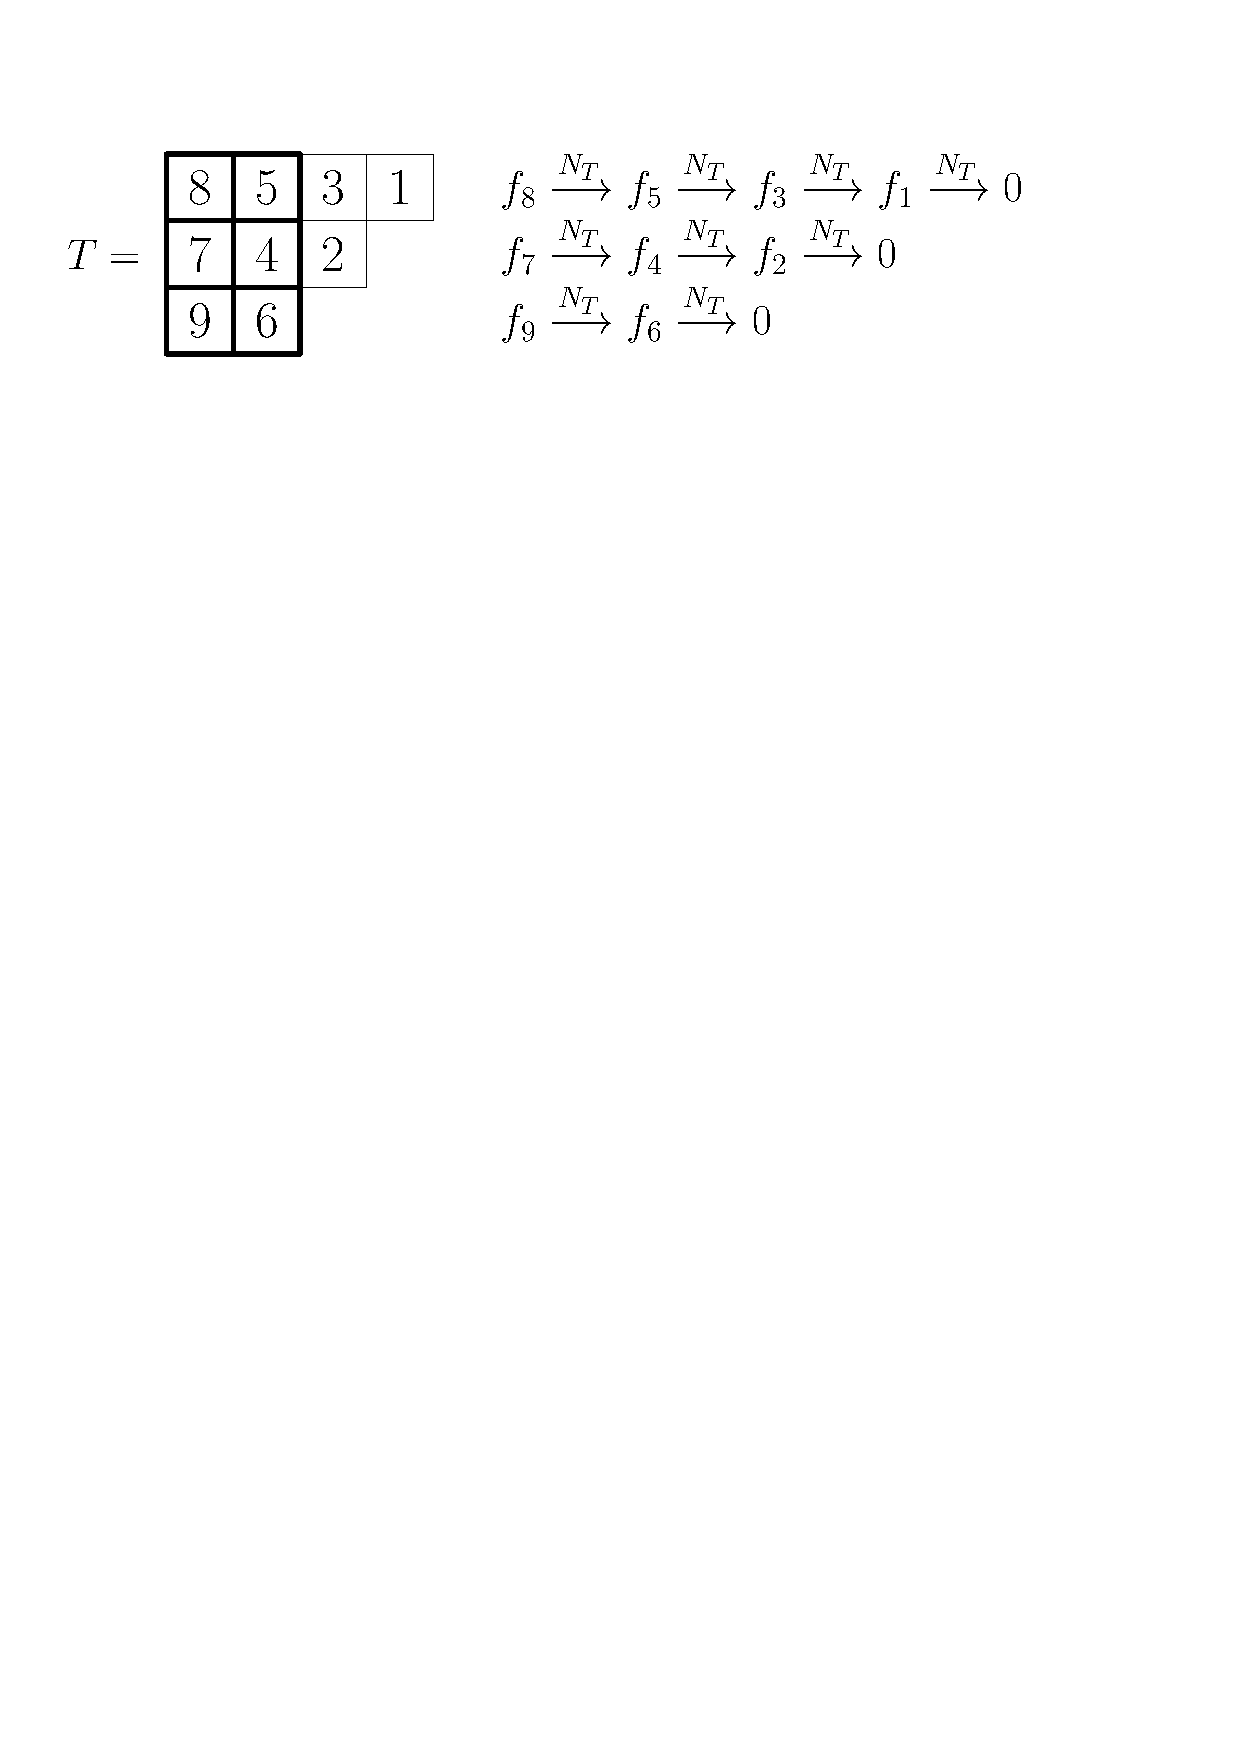
\includegraphics[width=0.7\textwidth]{Figures/SchubertCompatible.pdf}
    \caption{A Schubert-compatible filling $T$ of $\Lambda(5,(2,1),3)$, and the action of $N_T$ on the basis vectors.}
    \label{fig:SchubertCompatible}
\end{figure}

\begin{example}
Let $n=5$, $\lambda = (2,1)$, and $s=3$. Let $T$ be the Schubert-compatible filling of $\Lambda(5,(2,1),3)$ in Figure~\ref{fig:SchubertCompatible}. Then $Y_{5,(2,1),3}$ is the variety of partial flags $V_\bullet = (V_1,V_2,V_3,V_4,V_5)\in \Fl_{(1,1,1,1,1)}(\bC^9)$ such that the following conditions hold:
\begin{align}
N_T V_i &\subseteq V_{i} \text{ for } i \leq 5, \\
% N V_4\subseteq V_3,\, NV_3\subseteq V_2,\, NV_2\subseteq V_1,\, NV_1\subseteq 0,\\
V_5 &\supseteq F_3 = \vspan\{f_1,f_2,f_3\}.
\end{align}
For example, the partial flag 
\begin{equation*}\label{eq:PartialFlag}
\vspan\{ f_1 \} \subset \vspan\{ f_1,f_2 \} \subset 
\vspan\{ f_{1},f_{2},f_{4} \} \subset \vspan\{ f_{1},f_{2},f_{3},f_{4} \} \subset \vspan\{ f_{1},f_{2},f_{3},f_{4},f_{7}\}.
\end{equation*}
is in $Y_{5,(2,1),3}$.
\end{example}


\begin{example}\label{ex:ReadingOrder}
We construct a Schubert-compatible filling $T$ as follows. 
Let the \emph{reading order} of $[\Lambda]$ be the ordering of the cells given by scanning down the columns of $[\Lambda]$ from right to left. For $(i,j)\in [\Lambda]$, if $(i,j)$ is the $p$th cell in the reading order, then let $T(i,j)=p$. It can be checked that $T$ is a Schubert-compatible filling. See the left-most filling in Figure~\ref{fig:ReadingOrder} for an example of such a filling with $n=7$, $\lambda = (2,2)$, and $s=4$.
\end{example}

\begin{lemma}\label{lem:S6}
Suppose $T$ is a Schubert-compatible filling. If $j<\Lambda_i$, then \[N_T (F_{T(i,j)}\setminus F_{T(i,j)-1}) \subseteq F_{T(i,j+1)}\setminus F_{T(i,j+1)-1}.\]
\end{lemma}

\begin{proof}
We have $N_T \, f_{T(i,j)} = f_{T(i,j+1)}$ by definition. Let $f_{T(a,b)}\in F_{T(i,j)}$ with $T(a,b) < T(i,j)$. If $b<\Lambda_a$, then since $T(a,b) < T(i,j)$, by (S6) we have $T(a,b+1) < T(i,j+1)$, and hence $N_T\, f_{T(a,b)} = f_{T(a,b+1)}\in F_{T(i,j+1)}$. Otherwise, if $b=\Lambda_a$, then $N_T\, f_{T(a,b)} = 0$. In either case, we have $N_T F_{T(i,j)} \subseteq F_{T(i,j+1)}$. 

If $v\in F_{T(i,j)}\setminus F_{T(i,j)-1}$, then the expansion of $v$ in the $f$ basis has a nonzero $f_{T(i,j)}$ coefficient. Therefore, the expansion of $N_T\, v$ in the $f$ basis has a nonzero $f_{T(i,j+1)}$ coefficient, so $N_T\, v\notin F_{T(i,j+1)-1}$. The lemma then follows.
\end{proof}



For $1\leq i \leq s$, define a {\bf flattening function} $\fl_T^{(i)}$ 
%and its inverse $\ufl^{(i)}$ \tcr{(do we really need separate notation for the inverse?)}, partitions $\Lambda^{(i)}$ and $\lambda^{(i)}$, 
and a filling $T^{(i)}$ as follows.
If $i\leq \ell(\lambda)$, then $\fl_T^{(i)}$ is the unique order-preserving function with the following domain and codomain,
\begin{align}
    \fl_T^{(i)} : [K]\setminus\{ T(i,\Lambda_i) \} \to [K-1],
\end{align}
and if $i> \ell(\lambda)$, then $\fl_T^{(i)}$ is the unique order preserving function
\begin{align}
    \fl_T^{(i)}: [K]\setminus(\{T(i,\Lambda_i)\}\cup \{T(i',1)\mid i'\neq i\}) \to [K-s].
\end{align}
For $i\leq \ell(\lambda)$, let $T^{(i)}$ be the filling obtained by deleting the last box in row $i$, applying $\fl_T^{(i)}$ to the label in each cell, and reordering the rows so that the labels of the cells in the new right edge are increasing from top to bottom.
For $i>\ell(\lambda)$, we also delete each cell $(i',1)$ for $i'\neq i$ and shift row $i'$ to the left by one unit before applying $\fl_T^{(i)}$ to form $T^{(i)}$.

See Figure~\ref{fig:ReadingOrder} for an example of a Schubert-compatible filling $T$ and the fillings $T^{(1)}$ and $T^{(3)}$. When constructing $T^{(3)}$, the cells labeled by $7,13,14$, and $16$ are deleted, and rows $1,2$ and $4$ are shifted left by one unit. The cells are relabeled as follows: $\fl_T^{(3)}(8)=7$, $\fl_T^{(3)}(9) = 8$, $\fl_T^{(3)}(10) = 9$, $\fl_T^{(3)}(11)=10$, $\fl_T^{(3)}(12) = 11$, and $\fl_T^{(3)}(15)=12$. Then rows $3$ and $4$ are swapped to obtain $T^{(3)}$. It can be checked that both $T^{(1)}$ and $T^{(3)}$ are  Schubert compatible.

\begin{lemma}
If $i \leq \ell(\lambda)$, then $T^{(i)}$ is $(n-1,\lambda^{(i)},s)$-Schubert compatible. If $i > \ell(\lambda)$, then $T^{(i)}$ is $(n-1,\lambda,s)$-Schubert compatible.
\end{lemma}

\begin{proof}
By (S4), the labeling $T^{(i)}$ is of partition shape after sorting the rows by the labels in the right edge. It is immediate from the definitions that if $i\leq \ell(\la)$ then $T^{(i)}$ is of shape $\Lambda(n-1,\la^{(i)},s)$ and if $i> \ell(\la)$, then $T^{(i)}$ is of shape $\Lambda(n-1,\la,s)$. It also follows by construction that (S1) and (S2) hold for $T^{(i)}$.

Since the operations of deleting a cell, applying the flattening function to the labels, and possibly shifting a row to the left all preserve (S3), then $T^{(i)}$ has property (S3). Since (S4) only concerns labels of $[\lambda]$, and all cells of $[\lambda]$ are shifted left during the process of constructing $T^{(i)}$, then $T^{(i)}$ also satisfies (S4). The property (S5) is automatically satisfied by construction. Finally, $T^{(i)}$ satisfies (S6) since deleting a cell, relabeling, swapping rows, and shifting a row to the left all preserve the property (S6). Therefore, $T^{(i)}$ is Schubert compatible. 
\end{proof}




\begin{figure} 
    \centering
    \includegraphics[width=0.7\textwidth]{Figures/ReadingOrder.pdf}
    \caption{The Schubert-compatible filling $T$ of $[\Lambda] = [\Lambda(7,(2,2),4)]$ determined by reading order and the fillings $T^{(1)}$ and $T^{(3)}$, which are also Schubert compatible.}
    \label{fig:ReadingOrder}
\end{figure}


%Given a Schubert-compatible filling $T$, define functions $s_T : [K]\to \bZ_{\geq 0}$ and $p_T : [K]\to \bZ_{\geq 0}$ as follows. Given $a\leq K$, let $(i,j) = T^{-1}(a)$. Define $s_T(a)=T(i,j+1)$ and $p_T(a)=T(i,j-1)$, where by convention we declare that $T(i',j')$ is $0$ if $(i',j')\notin \Lambda$.  (We want $s_T(a)=0$ if $a$ is in the last box?)


The set of injective maps $w:[n]\rightarrow [K]$ indexes the Schubert cells of $\Fl_{(1^n)}(\mathbb{C}^K)$.
Given such a map, we say that $w$ is {\bf admissible} with respect to $T$ if both of the following hold.
\begin{itemize}
    \item[(A1)] The image of the map $w$ contains $[k]$.%\subseteq \{w(i)\mid i\in [n]\}$
    \item[(A2)] For $i\leq n$, if $w(i)=T(a,b)$ for $b<\Lambda_a$, then $T(a,b+1)\in \{w(1),\dots, w(i-1)\}$. 
\end{itemize}

\begin{lemma}\label{lem:NonemptyIntersections}
Assume $T$ is a Schubert-compatible filling.  Then  $C_w\cap Y_{T}\neq\emptyset$ if and only if $w$ is admissible.
\end{lemma}



\begin{proof}
If $w$ is admissible, then the partial flag $V_\bullet$ defined by $V_i=\langle f_{w(1)}, \ldots, f_{w(i)}\rangle$ is in $C_w\cap Y_{T}$, so $C_w\cap Y_{T} \neq \emptyset$. Therefore, it suffices to prove that if $C_w\cap Y_{T}\neq\emptyset$, then $w$ is admissible.

Given an injective map $w: [n]\to [K]$, recall that 
\begin{align}
    C_w = \{V_\bullet \in \Fl_{(1^n)}(\bC^K) \st \dim(V_i\cap F_j) = \#\{p\leq i \st w(p)\leq j\}\}.
\end{align}
Given $V_\bullet\in \Fl_{(1^n)}(\bC^K)$, then $F_k\subseteq V_n$ if and only if $\dim(V_n\cap F_k) = k$. Therefore, $F_k\subseteq V_n$ for some $V_\bullet\in C_w$ if and only if (A1) holds.

Suppose $C_w\cap Y_{T}\neq\emptyset$, and let $V_\bullet \in C_w\cap Y_{T}$. Suppose there exists a $i\leq n$ such that $w(i) = T(a,b)$ with $b<\Lambda_a$.
Then $\dim(V_i\cap F_{T(a,b)})>\dim(V_i\cap F_{T(a,b)-1})$, so $V_i\cap (F_{T(a,b)}\setminus F_{T(a,b)-1})\neq\emptyset$.  By Lemma~\ref{lem:S6}, we have $N_T (F_{T(a,b)}\setminus F_{T(a,b)-1}) \subseteq F_{T(a,b+1)}\setminus F_{T(a,b+1)-1}$. Hence,
\begin{align}
    N_T V_i \cap (F_{T(a,b)} \setminus F_{T(a,b+1)-1}) \neq \emptyset
\end{align}
and since $N_T V_i\subseteq V_{i-1}$, then
\begin{align}
    V_{i-1} \cap (F_{T(a,b+1)}\setminus F_{T(a,b+1)-1}) \neq \emptyset,
\end{align}
so $T(a,b+1)=w(i')$ for some $i'\leq i-1$. Hence, (A2) holds and $w$ is admissible.
\end{proof}

We define a linear transformation related to $N_T$ that we use throughout the paper.
\begin{definition}\label{def:NTranspose}
Define the nilpotent endomorphism $N^t_T$ of $\bC^K$ on the basis $\{f_1,\dots, f_K\}$ as follows,
\begin{align}
N^t_T \,f_{T(i,j)} \coloneqq \begin{cases} f_{T(i,j-1)} & \text{ if } j>1,\\ 0 & \text{ if }j = 1.\end{cases}
\end{align}
\end{definition}
Our notation is motivated by the fact that the matrix for $N^t_T$ with respect to the ordered basis $\{f_i\}$ is the transpose of the matrix for $N_T$. The transformation $N^t_T$ has the crucial property that 
\begin{align}\label{eq:NNTranspose}
N_TN^t_T \,f_{T(i,j)} = \begin{cases} f_{T(i,j)} &\text{ if } j > 1\\ 0 &\text{ if } j = 1.\end{cases}
\end{align}




\begin{lemma}\label{lem:InvertibleTransf}
Let $T$ be Schubert compatible, $w$ be admissible, and $w(1) = T(i,\Lambda_i)$. Given $v\in \vspan\{f_{T(h,\Lambda_h)}\st h<i\}$, then the linear transformation $U_v: \bC^K\to \bC^K$ defined by
\begin{align}
    U_v(f_{T(p,q)}) = \begin{cases} f_{T(p,q)} + (N^t_T)^{\Lambda_i-q}\,v & \text{ if }p=i\\ f_{T(p,q)} & \text{ otherwise.}\end{cases}
\end{align}
is upper triangular with $1$s along the diagonal such that $N_TU_v = U_vN_T$.
\end{lemma}

\begin{proof}
In the case $p=i$, the nonzero components of the vector $(N_T^t)^{\Lambda_i-q}\,v$ are $f_{T(j,\Lambda_j-(\Lambda_i-q))}$ for $j<i$. By (S5), we have $T(j,\Lambda_j) < T(i,\Lambda_i)$ for all $j<i$. Therefore, by applying (S6) $\Lambda_i-q$ many times, we have $T(j,\Lambda_j-(\Lambda_i-q)) < T(i,q)=T(p,q)$. Hence, $T_v$ is upper triangular with $1$s along the diagonal.

Given $f_{T(p,q)}$ such that $p\neq i$, then $N_T U_v f_{T(p,q)} = N_T f_{T(p,q)} = U_v N_T f_{T(p,q)}$, where the second equality follows from the fact that either $N_T f_{T(p,q)} = f_{T(p,q+1)}$ or $0$. On the other hand, if $p=i$, then 
\begin{align}
    U_v N_T f_{T(i,q)} = \begin{cases} f_{T(i,q+1)} + (N_T^t)^{\Lambda_i-q-1}v & \text{ if } q<\Lambda_i\\  0 & \text{ if }q = \Lambda_i,\end{cases}
\end{align}
Likewise, we have
\begin{align}
    N_T U_v f_{T(i,q)} = N_T f_{T(i,q)} + N_T(N_T^t)^{\Lambda_i-q}v 
\end{align}

\begin{align}
    N_T U_v f_{T(i,q)} = N_T f_{T(i,q)} + (N_T N_T^t) (N_T^t)^{\Lambda_i-q-1}v = f_{T(i,q+1)} + (N_T^t)^{\Lambda_i-q-1}v,
\end{align}
where the second equality follows from~\eqref{eq:NNTranspose}. Hence, $N_TU_v = U_vN_T$ and the proof is complete.
\end{proof}


\begin{lemma}\label{lem:CellRecursion}
Let $T$ be Schubert compatible, $w$ be admissible, and $w(1)= T(i,\Lambda_i)$. We have 
\[C_w\cap Y_{T}\cong \mathbb{C}^{i-1}\times (C_{\fl_T^{(i)}(w)}\cap Y_{T^{(i)}}).\]
\end{lemma}

\begin{proof}
Since
\begin{align}
    \vspan\{f_{T(j,\Lambda_j)}\st j<i\} \cong \bC^{i-1},
\end{align}
we may identify the two spaces as affine varieties. Define linear maps
\begin{align}
    \psi^{(i)} : \bC^{K-1} \to \bC^K & \,\,\,\text{  for  }i\leq \ell(\la),\\
    \psi^{(i)} : \bC^{K-s} \to \bC^K & \,\,\,\text{  for  }i > \ell(\la),
\end{align}
by $\psi^{(i)}(f_j) \coloneqq f_{(\fl_T^{(i)})^{-1}(j)}$, and extend linearly. 
Given $v\in \vspan\{f_{T(j,\Lambda_j)}\st j<i\}$ and $V_\bullet\in C_{\fl_T^{(i)}(w)}\cap Y_{T^{(i)}}$, define $\Phi(v,V_\bullet)$ to be
\begin{align}
   (\vspan\{f_{w(1)}+v\},\vspan\{f_{w(1)}+v\} + U_v\psi^{(i)}(V_1), \dots, \vspan\{f_{w(1)}+v\} + U_v\psi^{(i)}(V_{n-1})).
\end{align}


\textbf{Claim:} The partial flag $\Phi(v,V_\bullet)$ is in $C_w\cap Y_T$, so $\Phi$ is a well-defined map
\begin{align}\label{eq:PhiIso}
 \Phi : \vspan\{f_{T(j,\Lambda_j)}\st j<i\} \times (C_{\fl_T^{(i)}(w)}\cap Y_{T^{(i)}}) \to C_w\cap Y_T.
 \end{align}

It can be checked that since $V_\bullet\in C_{\fl_T^{(i)}(w)}$, then $\Phi(0,V_\bullet) \in C_w$.
Observe that $\Phi(v,V_\bullet) = U_v\Phi(0,V_\bullet)$, where $U_v$ acts on each subspace in the partial flag $\Phi(0,V_\bullet)$. Since $U_v$ is upper triangular with $1$s along the diagonal by Lemma~\ref{lem:InvertibleTransf}, it preserves the Schubert cell $C_w$, so $\Phi(v,V_\bullet)\in C_w$. In particular, since $w$ is admissible then the $n$th part of the partial flag $\Phi(v,V_\bullet)$ contains $F_k$. Furthermore, it can be checked that $N_T\psi^{(i)}(w)-\psi^{(i)}N_T^{(i)}(w)\in \ker(N_T)$ for all $w$ in the domain of $\psi^{(i)}$. Combining this with Lemma~\ref{lem:InvertibleTransf}, we have
\begin{align}
    N_T(\vspan\{v\} + U_v\psi^{(i)}(V_j)) = N_TU_v\psi^{(i)}(V_j) = U_v\psi^{(i)}N_{T^{(i)}}(V_j) \subseteq U_v\psi^{(i)}(V_{j-1}).
\end{align}
Hence, $\Phi(v,V_\bullet)\in C_w\cap Y_T$, which proves the claim.

To show that $\Phi$ is an isomorphism, it suffices to show that $\Phi$ has an inverse. Define linear maps
\begin{align}
    \phi^{(i)} : \bC^K \to \bC^{K-1} & \,\,\,\text{  for  }i\leq \ell(\la),\\
    \phi^{(i)} : \bC^K \to \bC^{K-s} & \,\,\,\text{  for  }i>\ell(\la),
\end{align}
by $\Phi^{(i)}(f_j) \coloneqq f_{\fl_T^{(i)}(j)}$ if $j$ is in the domain of $\fl_T^{(i)}$ and $0$ otherwise.
Given $V_\bullet\in C_w\cap Y_T$, there exist unique vectors $v_1,\dots, v_n$ with $v_i\in V_i$ such that the coefficient of $f_{w(i)}$ in $v_i$ is $1$ and the coefficient of $f_{w(i)}$ in $v_j$ is $0$ for all $i<j$. Define $V_i' = \vspan\{v_2,\dots, v_{i+1}\}$ for all $i$. Then it can be checked that the inverse of $\Phi$ is 
\begin{align}
    \Phi^{-1}(V_\bullet) = (v_1-f_{w(1)}, (\phi^{(i)}U_{v_1-f_{w(1)}}^{-1}(V'_1),\dots,\phi^{(i)}U_{v_1-f_{w(1)}}^{-1}(V'_{n-1}))).
\end{align}
Moreover, since $U_v$ can be represented by a unipotent upper triangular matrix whose coordinates are regular functions on $Y_{T}$, then the same is true of $U_v^{-1}$, and hence both $\Phi$ and $\Phi^{-1}$ are algebraic maps, so $\Phi$ is an isomorphism of algebraic varieties.
\end{proof}

 

\begin{theorem}\label{thm:AffinePavingY}
If $T$ is Schubert compatible, then the intersections $C_w\cap Y_{n,\la,s,T}$ for $w$ admissible are the cells of an affine paving of $Y_{n,\la,s,T}$.
\end{theorem}

\begin{proof}
Since the Schubert cells $C_w$ are the cells of an affine paving of $\Fl_{(1^n)}(\bC^K)$, it suffices to show that each nonempty intersection $C_w\cap Y_{n,\la,s,T}$ is isomorphic to an affine space $\bC^d$ for some $d$. By Lemma~\ref{lem:CellRecursion}, $C_w\cap Y_{n,\la,s,T}$ is nonempty if and only if $w$ is admissible. We proceed by induction on $n$ to show that each of these intersection is an affine space. In the base case when $n=1$, either $\lambda =\emptyset$ or $\lambda = (1)$. In the first case, $Y_{1,\emptyset,s,T} = \bP^{s-1}$ for any Schubert-compatible $T$, the admissible $w$ are in bijection with $[s]$, and the nonempty intersections $C_w\cap Y_{1,\emptyset,s,T}$ can be identified with usual cells of $\bP^{s-1}$. In the second case, $Y_{1,(1),s,T}$ is a point, and the only nonempty intersection is a point. The inductive proof then follows by applying Lemma~\ref{lem:CellRecursion}.
\end{proof}

\begin{figure}[t]
  \centering
  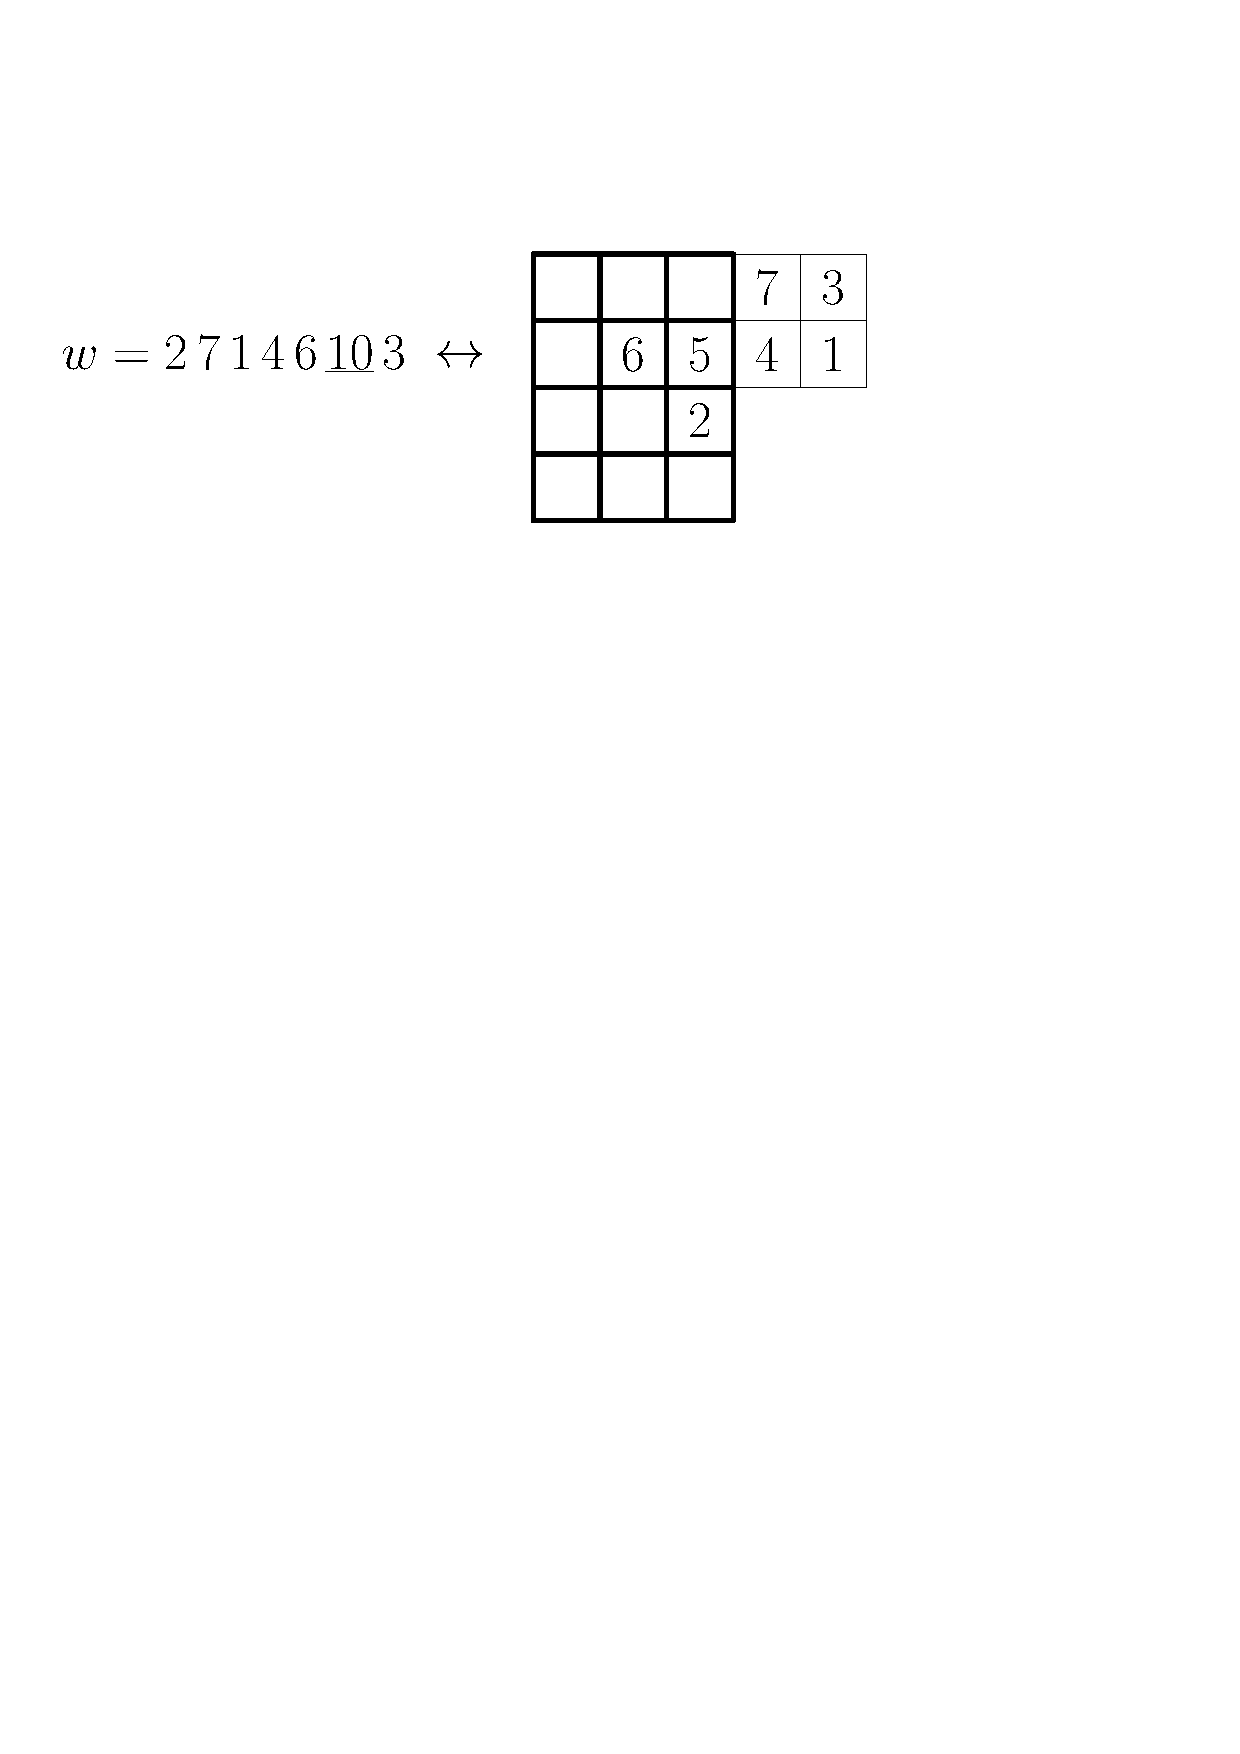
\includegraphics[scale=0.6]{Figures/RowDecreasingBijection.pdf}
  \caption{With $T$ as in Figure~\ref{fig:ReadingOrder}, an example of the bijective correspondence in the proof of Theorem~\ref{thm:AffinePavingY}.\label{fig:FillingBijectionExample}}
\end{figure}

\begin{corollary}\label{cor:AffinePavingFillings}
The cells in an affine paving of $Y_{n,\la,s,T}$ are in bijection with partial fillings of $[\Lambda]$ that decrease from left to right along each row and such that the labels in each row are right justified and every cell of $[\lambda]$ is filled.
\end{corollary}

\begin{proof}
By Theorem~\ref{thm:AffinePavingY}, the cells in an affine paving of $Y_{n,\la,s,T}$ are in bijection with injective functions $w$ that are admissible with respect to $T$. The admissible injective functions are in bijection with the set of partial fillings in the statement of the corollary under the following map. Given an admissible $w$, for $1\leq i\leq n$, if $w(i) = T(a,b)$, then label the cell $(a,b)$ of $\Lambda$ with $w(i)$. It can be checked that this defines a bijection between the two sets. See Figure~\ref{fig:FillingBijectionExample} for an example of this correspondence.
\end{proof}



\begin{remark}
  Recall that in the case where $\la=(1^k)$ and $s=k$, the ring $R_{n,\la,s}$ specializes to the Haglund--Rhoades--Shimozono ring, $R_{n,(1^k),k} \cong R_{n,k}$. This ring has a $\bZ$-basis indexed by \emph{ordered set partitions}, which are partitions of the set $[n]$ into a $k$-tuple of nonempty blocks $(B_1,\dots, B_k)$. Part of the motivation that led us to define the variety $Y_{n,\la,s}$ was the following bijection between ordered set partitions and cells of $Y_{n,(1^k),k}$. Fix a Schubert compatible $T$. Given $w$ admissible with respect to $T$, let $P$ be the partial filling of $[\Lambda]$ corresponding to $w$ under the bijection defined in the proof of Theorem~\ref{cor:AffinePavingFillings}. Map $P$ to the ordered set partition $(B_1,\dots, B_k)$ where block $B_i$ is defined to be the set of labels in the $i$th row of $P$. It can be checked that this map defines the desired bijection. Hence, the total rank of $H^*(Y_{n,(1^k),k})$ is equal to the rank of $R_{n,k}$.

  For example, let $n=6$ and $k=3$, and let $T$ be the Schubert-compatible filling of $\Lambda(5,(1^2),2)$ according to reading order,
  \[
    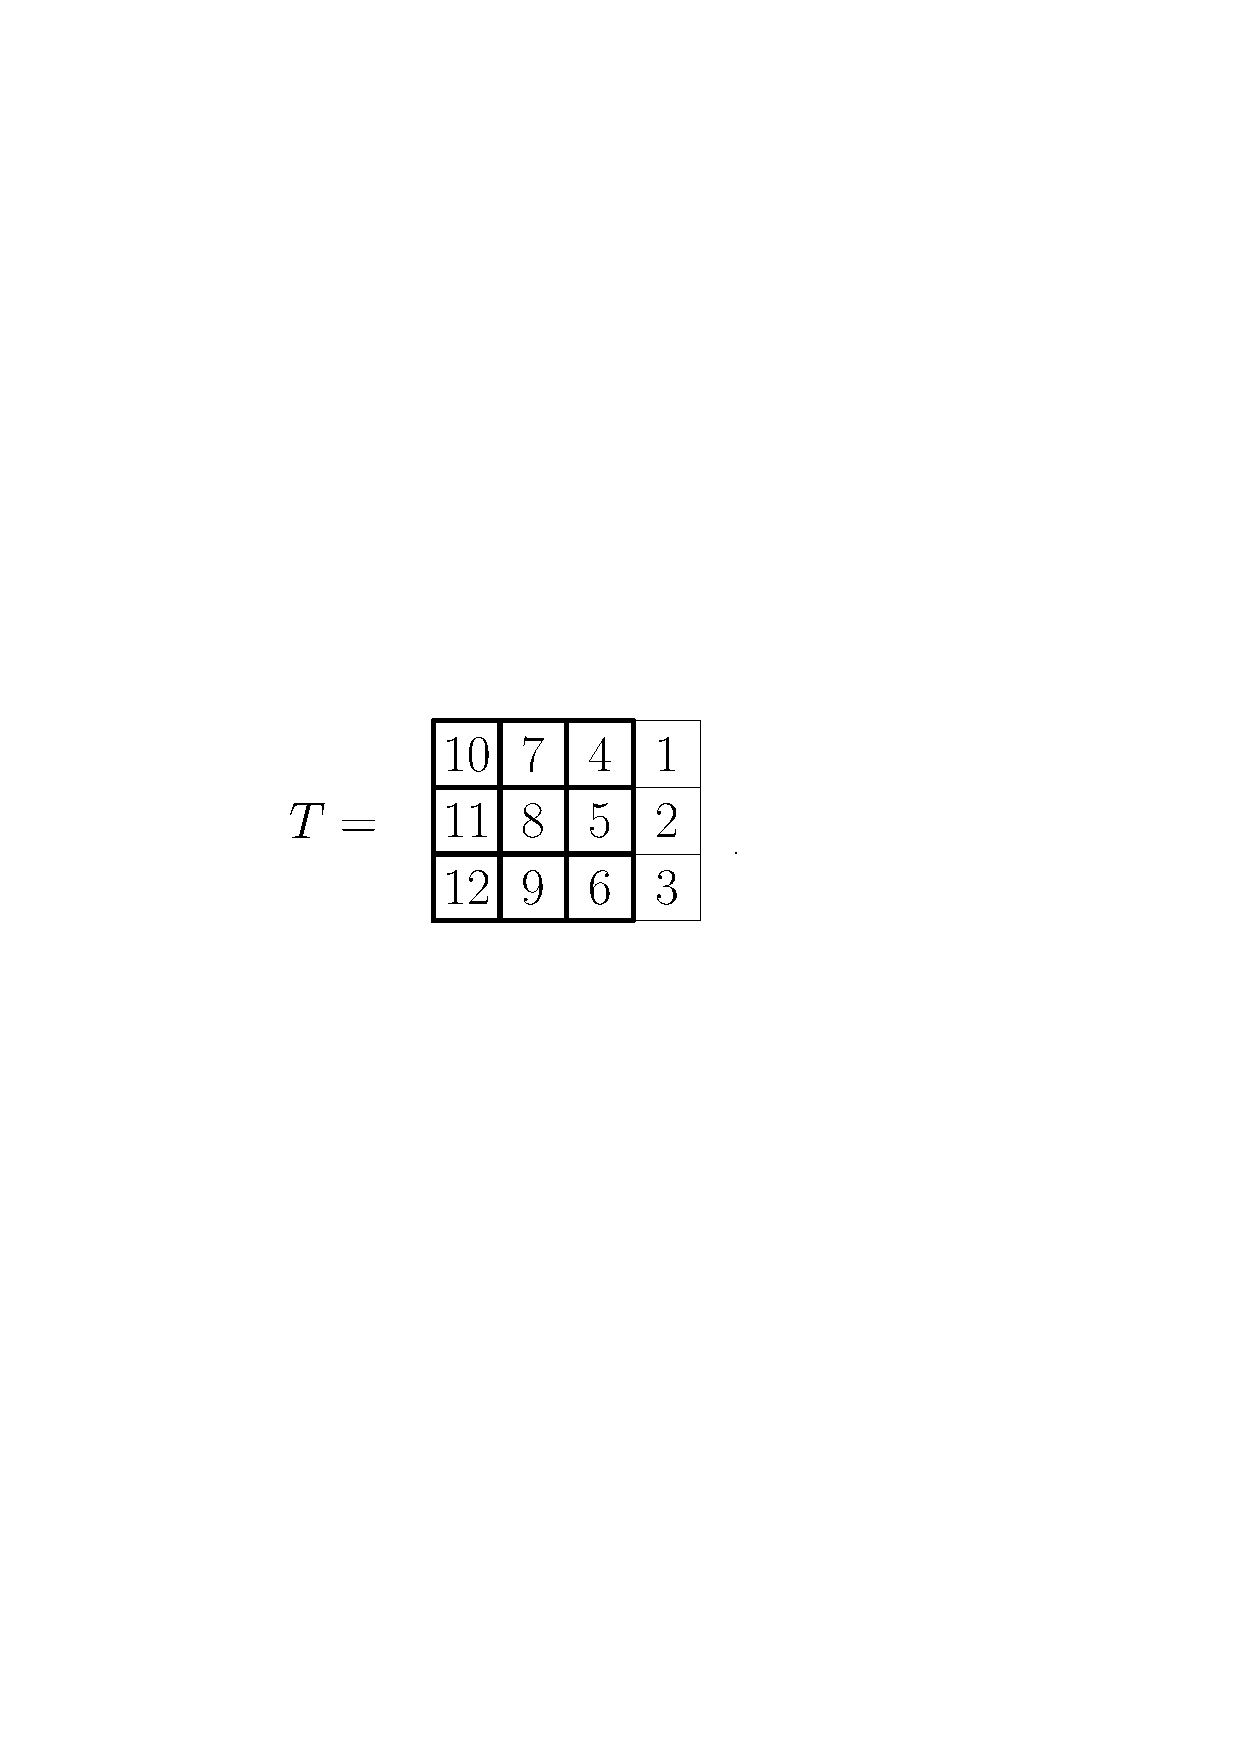
\includegraphics[scale=0.6]{Figures/OSPSchubertCompatible.pdf}
  \]
  Then the image of $w=253618$ under this correspondence is
  \[
    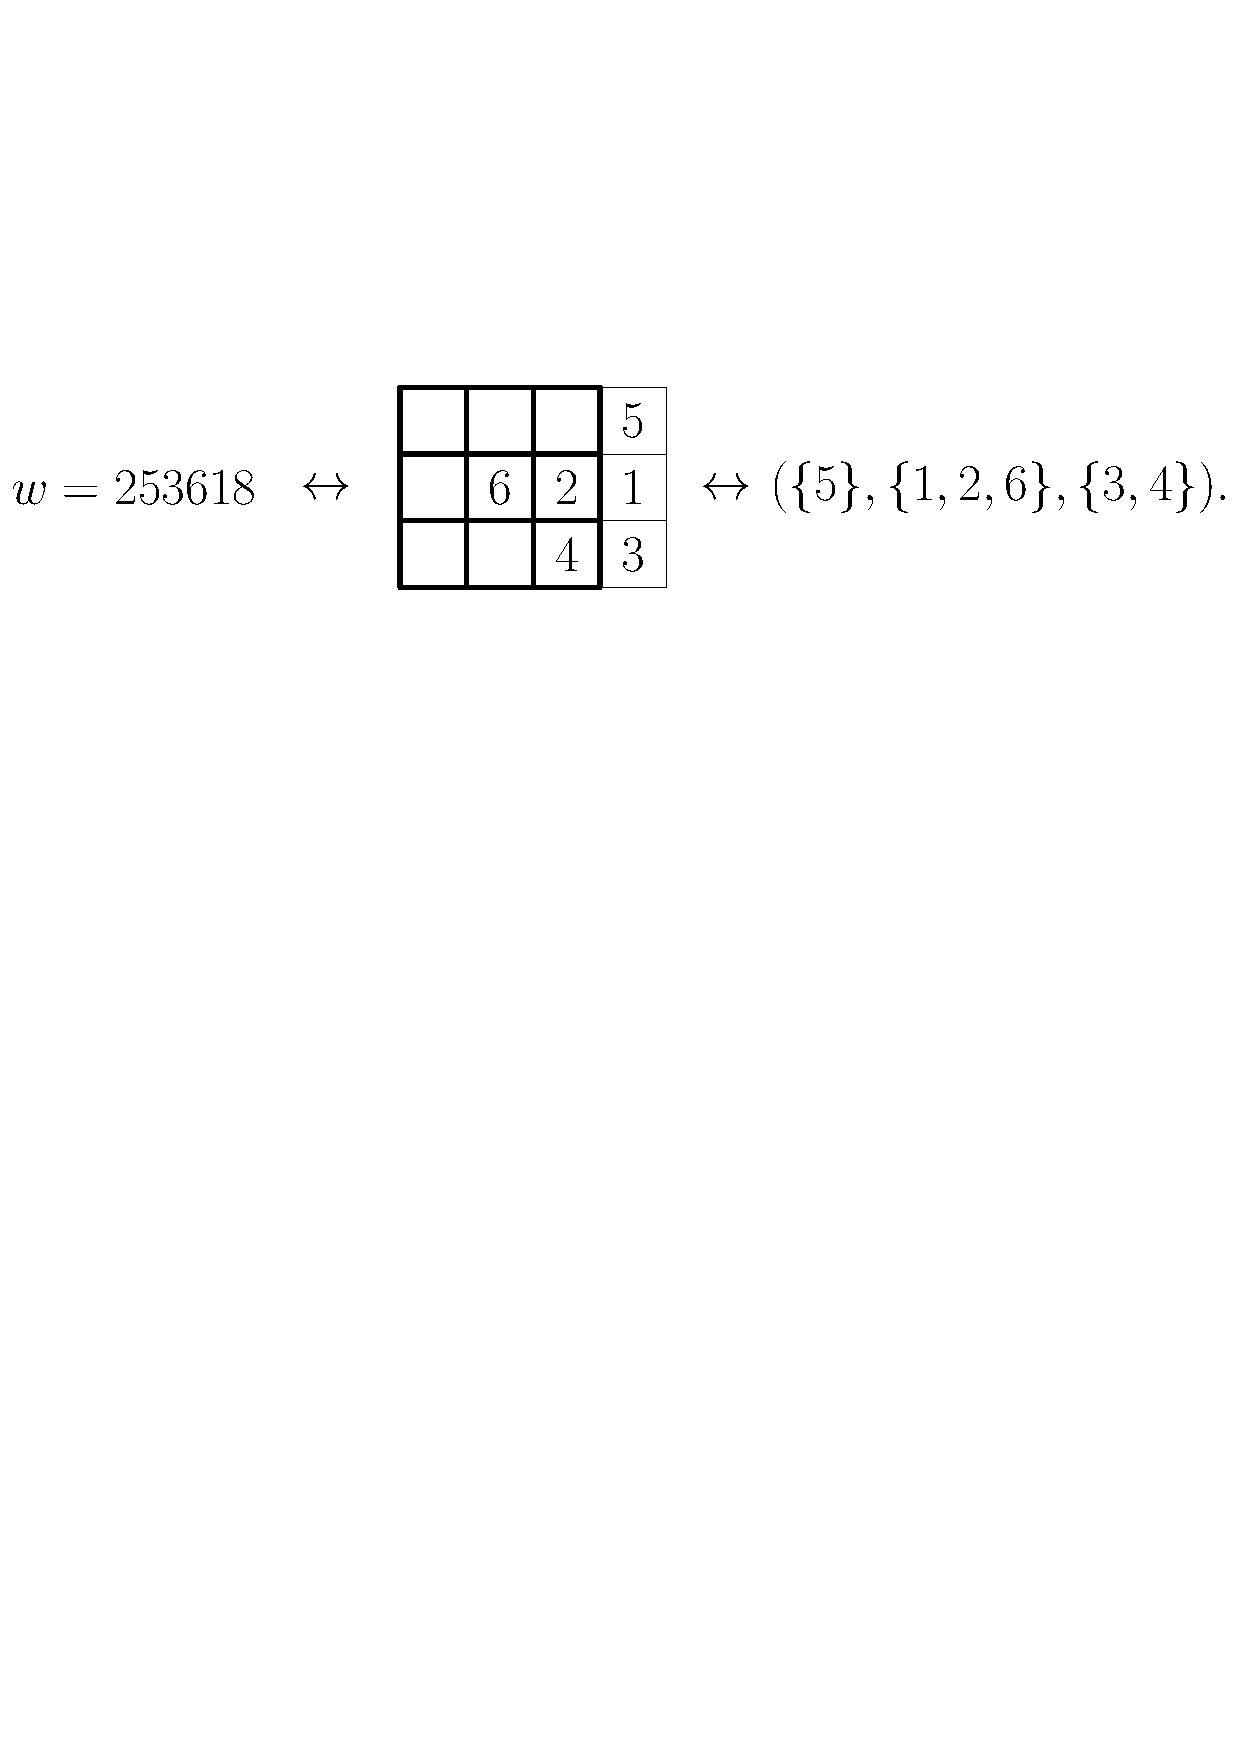
\includegraphics[scale=0.6]{Figures/OSPBijection.pdf} 
  \] 
\end{remark}

\begin{corollary}\label{cor:CohHilbRecursion}
We have
\[
\Hilb(H^*(Y_{n,\la,s});q) = \sum_{i=1}^{\ell(\la)} q^{2(i-1)} \Hilb(H^*(Y_{n-1,\la^{(i)},s});q) + \sum_{i=\ell(\la)+1}^s q^{2(i-1)} \Hilb(H^*(Y_{n-1,\la,s});q).
\]
\end{corollary}

\begin{proof}
Let $T$ be Schubert compatible. By Lemma~\ref{lem:OddCohVanishes}, the $q^{2i}$ coefficient of $\Hilb(H^*(Y_{n,\la,s});q)=\Hilb(H^*(Y_{n,\la,s,T});q)$ is the number of cells $C_w\cap Y_{n,\la,s,T}$ for $w$ admissible that are complex dimension $i$. It can be checked that for $1\leq i\leq s$, then $\{\fl^{(i)}(w) \st w\text{ admissible}\}$ is the set of admissible injective maps for $T^{(i)}$. Thus, the subspaces $C_{\fl^{(i)}(w)}\cap Y_{T^{(i)}}$ are the cells of an affine paving for $Y_{T^{(i)}}$, by Theorem~\ref{thm:AffinePavingY}.  The corollary then follows from Lemma~\ref{lem:CellRecursion}.
\end{proof}

\begin{corollary}\label{cor:RankGenNLaS}
The cohomology ring $H^*(Y_{n,\la,s,T})$ is a graded free $\bZ$-module concentrated in even degrees, whose rank generating function is equal to $\Hilb(R_{n,\la,s};q^2)$.
\end{corollary}
\begin{proof}
By Theorem~\ref{thm:AffinePavingY}, $Y_{n,\la,s,T}$ has a paving by affines where each cell is a copy of complex affine space. By Lemma~\ref{lem:OddCohVanishes}, all of the odd cohomology group vanish, and $H^{2i}(Y_{n,\la,s,T})$ is a free $\bZ$-module of rank equal to the number of cells of complex dimension $i$ in the paving.

We prove that the cohomology ring of $Y_{n,\la,s,T}$ and $R_{n,\la,s}$ have the same rank generating function by induction on $n$. In the case when $n=1$, then either $\la = \emptyset$ and $Y_{1,\emptyset,s,T} = \bP^{s-1}$, or $\la = (1)$ and $Y_{1,(1),s,T} = \bP^0$. In the first case, the rank generating function of $H^*(Y_{1,\emptyset,s,T})$ is $1 + q^2 +\dots + q^{2(s-1)}$. On the other hand, $R_{1,\emptyset,s} = \bZ[x]/(x^s)$, so the lemma holds in this case. In the second case, the rank generating function of $H^*(Y_{1,(1),s,T})$ is $1$, and $R_{1,(1),1}$ is the trivial $1$-dimensional ring, so the lemma holds in the base case.

Suppose $n>1$. By Lemma~\ref{lem:RHilbRecursion} and Corollary~\ref{cor:CohHilbRecursion}, the Hilbert series of $R_{n,\la,s}$ and the Hilbert series of $H^*(Y_{n,\lambda,s})$ satisfy the same recursion. Hence, the two $q$-series must be equal by induction on $n$. 
\end{proof}

\begin{lemma}\label{lem:Embedding}
Let $T$ be a $(n,\la,s)$-Schubert-compatible filling of $\Lambda(n,\la,s)$, and let $T'$ be a $(n,\emptyset,s)$-Schubert-compatible filling of $\Lambda(n,\emptyset,s) = (n^s)$ such that every entry of the $i$th row of $T$ is in the $i$th row of $T'$. Then the linear map $j : \bC^K \hookrightarrow \bC^{ns}$, which is the inclusion of the first $K$ coordinates, induces a closed embedding 
\begin{align}
\iota : Y_{n,\la,s,T}\hookrightarrow Y_{n,\emptyset,s,T'},
\end{align}
defined by sending the flag $V_\bullet\in Y_{n,\la,s,T}$ to the flag $(j(V_1),\dots, j(V_n))$.
\end{lemma}

\begin{proof}
The proof follows from the fact that the entries of $T$ in row $i$ are right justified in row $i$ of $T'$. \SG{What details should we add?}
\end{proof}

\begin{lemma}\label{lem:AffinePavingDiff}
If $T$ is a Schubert-compatible filling, the space $Y_{n,\emptyset,s,T'}\setminus \iota(Y_{n,\la,s,T})$ has an affine paving.
\end{lemma}

\begin{proof}
By Theorem~\ref{thm:AffinePavingY}, the intersections $C_w\cap Y_{n,\la,s,T}$ for $w$ admissible with respect to $T$ are the cells of an affine paving of $Y_{n,\la,s,T}$, and the intersections $C_v\cap Y_{n,\emptyset,s}$ for $v$ admissible with respect to $T'$ are the cells of an affine paving of $Y_{n,\emptyset,s,T'}$.

Given such a cell $C_w\cap Y_{n,\la,s,T}$ with $w$ admissible with respect to $T$, define $w' : [n]\to [ns]$ by extending the codomain of $w$ to $[ns]$. Then $w'$ is admissible with respect to $T'$, and it can be checked that $\iota(C_w\cap Y_{n,\la,s,T}) = C_{w'}\cap Y_{n,\emptyset,s,T'}$. Therefore, $Y_{n,\emptyset,s,T'}\setminus \iota(Y_{n,\la,s,T})$ has an affine paving given by removing the cells of the form $C_{w'}\cap Y_{n,\emptyset,s,T'}$ from the affine paving of $Y_{n,\emptyset,s,T'}$.
\end{proof}





\begin{corollary}\label{cor:Surj}
The closed embedding $\iota$ induces a surjection on cohomology,
\begin{align}
H^*(Y_{n,\emptyset,s,T}) \twoheadrightarrow H^*(Y_{n,\la,s,T'}).
\end{align}
\end{corollary}
\begin{proof}
This follows immediately by Lemma~\ref{lem:PavingSurj}, Theorem~\ref{thm:AffinePavingY}, and Lemma~\ref{lem:AffinePavingDiff}.
\end{proof}




% %%%%%%%%%%%%%%%%%%%%%%%%%%%%
% \section{Old affine paving of $Y_{n,\lambda,s}$}
% %%%%%%%%%%%%%%%%%%%%%%%%%%%%

% In this section, we define the variety $Y_{n,\la,s}$, and we prove that it has a paving by affines. Moreover, we prove that every $Y_{n,\la,s}$ embeds as a closed subvariety of $Y_{n,\emptyset,s}$ and that the affine paving is compatible with this closed embedding.

% The variety $Y_{n,\lambda,s}$ is defined as follows. Fix integers $0\leq k\leq n$ (with $n>0$), a partition $\lambda\vdash k$, and an integer $s\geq \ell(\lambda)$. Define $m = k + s(n-k)$, and let $\Fl_{1,\dots, n}(\bC^m)$ be the partial flag variety of ascending chains of subspaces $V_1\subset V_2\subset \cdots \subset V_n\subset \bC^m$ with $\dim_\bC(V_i) = i$ for all $i$. Fix a nilpotent endomorphism $N$ of $\bC^m$ whose matrix has Jordan type $(\la_1+n-k,\la_2+n-k,\dots, \la_s+n-k)$, where $\la_i \coloneqq 0$ for $i>\ell(\la)$. We define
% \begin{align}
% Y_{n,\la,s} \coloneqq \{V_\bullet \in \Fl_{1,\dots, n}(\bC^m) \st N V_i\subseteq V_{i-1}\text{ for all }i,\text{ and } V_n\supseteq \im(N^{n-k})\}.
% \end{align}
% When $k=n$, it can be checked that $Y_{n,\lambda,s} = \cB^\lambda$.

% Throughout the paper, we fix a basis of $\bC^m$,
% \begin{align}
% \{f_{i,j} \st i\leq s,\, j\leq \la_i+n-k\},
% \end{align}
%  such that $Nf_{i,j} = f_{i,j-1}$ for all $j>1$ and $Nf_{i,1} = 0$. The span of the vectors $f_{i,j}$ for a fixed $i$ is called a \emph{generalized eigenspace of $N$}.
 
 


% There is a filtration of $Y_{n,\la,s}$ by closed subvarieties $Y^1_{n,\la,s}\subseteq Y^2_{n,\la,s}\subseteq\cdots \subseteq Y^s_{n,\la,s}$, defined as follows. Observe that $\ker(N) = \vspan_\bC\{f_{1,1},\dots, f_{s,1}\}$. Let $F_\bullet$ be the complete flag of $\ker(N)$ given by $F_i = \vspan_\bC\{ f_{1,1},\dots, f_{i,1}\}$.
% For $i\leq s$, define
% \begin{align}
% Y_{n,\la,s}^i \coloneqq \{V_\bullet\in Y_{n,\la,s} \st V_1\subseteq F_i\},
% \end{align}
% where $Y_{n,\la,s}^0\coloneqq \emptyset$.
% Since $V_1\in \ker(N)$ for all $V_\bullet \in Y_{n,\la,s}$, we have $Y^s_{n,\la,s} = Y_{n,\la,s}$, so the subspaces $Y_{n,\la,s}^i$ form a filtration of $Y_{n,\la,s}$ by closed subvarieties.

% \begin{lemma}\label{lem:ProductIso}
% There is an isomorphism of varieties
% \begin{align}\label{eq:ProductIso}
% Y_{n,\la,s}^i \setminus Y_{n,\la,s}^{i-1} \cong \begin{cases} \bA^{i-1} \times Y_{n-1,\la^{(i)},s} & \text{if }1\leq i\leq \ell(\la)\\ \bA^{i-1}\times Y_{n-1,\la,s} & \text{if } \ell(\la)< i\leq s.\end{cases}
% \end{align}
% \end{lemma}

% \begin{proof}
% For any $i\leq s$, then $N$ induces a nilpotent transformation $N' : \bC^m/\langle f_{i,1}\rangle \to \bC^m/\langle f_{i,1}\rangle$. If $i\leq \ell(\la)$, then the Jordan type of $N'$ is
% \begin{align}
% (\la_1^{(i)} + n-k,\la_2^{(i)}+n-k,\dots, \la^{(i)}_s+n-k).
% \end{align}
% We then have an isomorphism of varieties
% \begin{align}
% \psi: \{V_\bullet \in Y_{n,\la,s} \st V_1 = \langle f_i\rangle \} \to Y_{n-1,\la^{(i)},s}
% \end{align}
% defined by $\psi(V_\bullet) = (V_2/\langle f_{i,1}\rangle,\dots, V_n/\langle f_{i,1}\rangle)$, which is a partial flag preserved by $N'$.

% If $\ell(\la) < i \leq s$, then $N'$ has Jordan type
% \begin{align}
% (\la_1+n-k,\dots,\la_{s-1}+n-k,\la_s+n-1-k).
% \end{align}
% By the same reasoning as in the first case, together with Lemma~\ref{lem:IsoWithLargerEmbedding}, we have an isomorphism
% \begin{align}
%  \{V_\bullet \in Y_{n,\la,s} \st V_1 = \langle f_i\rangle\} \cong Y_{n-1,\la,s}.
% \end{align}
% In order to prove the lemma, it suffices to prove
% \begin{align}\label{eq:ProdIsoWithDiff}
% F_{i-1}\times \{V_\bullet \in Y_{n,\la,s}\st V_1 = \langle f_{i,1}\rangle \} \cong Y_{n,\la,s}^i\setminus Y_{n,\la,s}^{i-1},
% \end{align}
% since $F_{i-1}\cong \bA^{i-1}$.


% Let $v$ be a vector in $F_{i-1}$. Define an invertible linear transformation $T_v : \bC^m \to \bC^m$ given by
% \begin{align}
% T_v(f_{i',j'}) = \begin{cases} f_{i',j'} +  (N^t)^{j'-1}\,v & \text{if } i'=i,\\ f_{i',j'} & \text{otherwise.}\end{cases}
% \end{align}
% For $(v,V_\bullet)\in F_{i-1}\times \{V_\bullet\in Y_{n,\la,s}\st V_1 = \langle f_i\rangle\}$, we claim that $(T_v(V_1),T_v(V_2),\dots, T_v(V_n))\in Y_{n,\la,s}^i \setminus Y_{n,\la,s}^{i-1}$. Indeed, by construction of $T_v$ we have $T_v(V_1)\in \bP(F_i)\setminus \bP(F_{i-1})$. The transformation $T_v$ preserves $\im(N^{n-k})$, so we have that $T_v(V_n) \supseteq \im(N^{n-k})$. Using \eqref{eq:NNTranspose}, it can be checked that $NT_v = T_v N$. Therefore, $NT_v(V_h) = T_v(NV_h) \subseteq T_v(V_{h-1})$ for all $h\leq n$, and hence $(T_v(V_1),\dots, T_v(V_n))\in Y_{n,\la,s}^i\setminus Y_{n,\la,s}^{i-1}$, as claimed. 

% Therefore, we have a map
% \begin{align}\label{eq:IsoWithSetDiff}
% \varphi : F_{i-1} \times \{V_\bullet \in Y_{n,\la,s} \st V_1 = \langle f_{i,1}\rangle\} \to Y_{n,\la,s}^i \setminus Y_{n,\la,s}^{i-1}
% \end{align}
% defined by $\varphi(v,V_\bullet) = (T_v(V_1),T_v(V_2),\dots, T_v(V_n))$. It follows from the definition of $T_v$ that it is represented by a matrix whose coordinates are regular functions on $Y_{n,\la,s}$. 
% Using the fact that $T_v$ is invertible, it can then be checked that $\varphi$ is an isomorphism of varieties, hence \eqref{eq:ProdIsoWithDiff} holds, and we are done.
% \end{proof}


% %%%% Definition of cell indexing %%%%%%%%
% Define an indexing of the cells in the affine paving of $Y_{n,\la,s}$ by sequences as follows. When $n=1$ and $\la = \emptyset$, let $C_{(i)} = \bP(F_i)\setminus \bP(F_{i-1})\cong \bA^{i-1}$. When $n=1$ and $\la = (1)$, let $C_1 = Y_{1,(1),s} \cong \bA^0$, a single point. 

% For $n>1$, suppose we have already indexed the cells of all $Y_{n-1,\la,s}$ as $C_{(i_1,\dots, i_{n-1})}$ for sequences $i_1,\dots, i_{n-1}\leq s$. For $i\leq s$, let $C_{(i_1,\dots, i_{n-1})}$ be the cell of $Y_{n-1,\la^{(i)},s}$ if $i\leq \ell(\la)$, or the cell of $Y_{n-1,\la,s}$ if $i > \ell(\la)$. Define $C_{(i_1,\dots, i_n)}$ to be the cell corresponding to $\bA^{i-1}\times C_{(i_1,\dots, i_{n-1})}$ under the isomorphism \eqref{eq:ProductIso}. Observe that
% \begin{align}\label{eq:DimOfCell}
% \dim_\bC (C_{(i_1,\dots, i_n)}) = \sum_{j\leq n} (i_j-1).
% \end{align}

% %%%%%%%%%%%%%%%%%%%%%%%%%%



% \begin{lemma}\label{lem:Embedding}
% Let $j : \bC^m \hookrightarrow \bC^{ns}$ be the inclusion of the first $m$ coordinates, and let $\widehat N$ be a nilpotent matrix with Jordan type $(n^s)$ that restricts to the nilpotent matrix $N$ on $\bC^m$. The linear map $j$ induces a closed embedding 
% \begin{align}
% \iota : Y_{n,\la,s}\hookrightarrow Y_{n,\emptyset,s},
% \end{align}
% defined by sending the flag $V_\bullet\in Y_{n,\la,s}$ to the flag $(j(V_1),\dots, j(V_n))$ preserved by $\widehat{N}$. 
% \end{lemma}

% \begin{proof}
% The fact that $\iota$ is an embedding follows by Lemma~\ref{lem:IsoWithLargerEmbedding}.
% \end{proof}





% \begin{theorem}\label{thm:AffinePavingNLaS}
% The spaces $Y_{n,\la,s}$ and $Y_{n,\emptyset,s}\setminus \iota(Y_{n,\la,s})$ have affine pavings. 
% \end{theorem}

% \begin{proof}
% We proceed by induction on $n$. In the base case when $n=1$, then either $\la = \emptyset$ and $Y_{1,\emptyset,s} = \bP^{s-1}$, or $\la = (1)$ and $Y_{1,(1),s} = \bP^0$, so the lemma holds. In the general case with $n>1$, then by our inductive hypothesis $Y_{n-1,\la^{(i)},s}$ and $Y_{n-1,\la,s}$ have affine pavings. By Lemma~\ref{lem:ProductIso}, then $Y_{n,\la,s}^i\setminus Y_{n,\la,s}^{i-1}$ is a disjoint union of affine subspaces $C_{(i_1,\dots, i_n)}$, and hence has a paving by affines.

% Given a cell $C_{(i_1,\dots, i_n)}$ of $Y_{n,\la,s}$, it can be checked that $\iota(C_{(i_1,\dots, i_n)}) = C_{(j_1,\dots, j_n)}$ for some $(j_1,\dots, j_n)$. \tcr{Should we actually say what the correspondence is? Or should we switch our notation so that the ``rows'' are given by a composition instead of a partition and fix it so that $\iota(C_{(i_1,\dots, i_n)}) = C_{(i_1,\dots, i_n)}$?}. Hence, $Y_{n,\emptyset,s}\setminus \iota(Y_{n,\la,s})$ has a paving by affines given by removing the image of each cell of $Y_{n,\la,s}$ under $\iota$.
% \end{proof}



% \begin{corollary}\label{cor:RankGenNLaS}
% The cohomology ring $H^*(Y_{n,\la,s})$ is a free $\bZ$-module concentrated in even degrees, whose rank generating function is equal to $\Hilb(R_{n,\la,s};q^2)$.
% \end{corollary}
% \begin{proof}
% By Theorem~\ref{thm:AffinePavingNLaS}, $Y_{n,\la,s}$ has a paving by affines where each cell is a copy of complex affine space. Therefore, all of the odd cohomology group vanish, and $H^{2i}(Y_{n,\la,s})$ is a free $\bZ$-module of rank equal to the number of cells of complex dimension $i$ in the paving, see e.g.~\cite{Hotta-Springer}.

% We prove that the rank generating function of the cohomology ring is equal to $\Hilb(R_{n,\la,s};q^2)$ by induction on $n$. In the case when $n=1$, then either $\la = \emptyset$ and $Y_{1,\emptyset,s} = \bP^{s-1}$, or $\la = (1)$ and $Y_{1,(1),s} = \bP^0$. In the first case, the rank generating function of $H^*(Y_{1,\emptyset,s})$ is $1 + q^2 +\dots + q^{2(s-1)}$. On the other hand, $R_{1,\emptyset,s} = \bZ[x]/(x^s)$, so the lemma holds in this case. In the second case, the rank generating function of $H^*(Y_{1,(1),s})$ is $1$, and $R_{1,(1),1}$ is the trivial $1$-dimensional ring, so the lemma holds in the base case.

% Let us assume that $n>1$. By \cite[Corollary 3.11]{GriffinOSP} and \cite[Theorem 3.18]{GriffinOSP}, the Hilbert series of $R_{n,\la,s}$ satisfies the following recursion,
% \begin{align}
% \Hilb(R_{n,\la,s};q^2) = \sum_{i=1}^{\ell(\la)} q^{2(i-1)} \Hilb(R_{n-1,\la^{(i)},s};q^2) + \sum_{i=\ell(\la)+1}^s q^{2(i-1)} \Hilb(R_{n-1,\la,s};q^2).
% \end{align}
% By Lemma~\ref{lem:ProductIso}, the rank generating function of $H^*(Y_{n,\la,s})$ satisfies the same recursion, hence the two $q$-series must be equal by induction.
% \end{proof}



% \begin{corollary}\label{cor:Surj}
% The closed embedding $\iota$ induces a surjection on cohomology,
% \begin{align}
% H^*(Y_{n,\emptyset,s}) \twoheadrightarrow H^*(Y_{n,\la,s}).
% \end{align}
% \end{corollary}
% \begin{proof}
% This follows immediately by Theorem~\ref{thm:AffinePavingNLaS} and Lemma~\ref{lem:PavingSurj}.
% \end{proof}



 
%
%
%\begin{lemma}\label{lem:XPowersVanish}
%Let $\widetilde{V}_i$ be the tautological rank $i$ vector bundle on $\Fl_{1,\dots, n}(\bC^m)$ pulled back to $Y_{n,\la,s}$, and let $x_i = -c_1(\widetilde{V}_i/\widetilde{V}_{i-1})$. Then we have $x_i^s=0$ for all $i$.
%\end{lemma}
%
%\begin{proof}
%This follows from Lemma~\ref{lem:CohEmptyPartition} and the naturality of Chern classes.
%\end{proof}
%



%
%\begin{lemma}\label{lem:JordanTypeRestriction}
%Let $\nu = (\la_1 + n-k,\dots, \la_s + n-k)$. Given $V_\bullet\in C_{(i_1,\dots, i_n)}\subseteq Y_{n,\la,s}$, the Jordan type of the nilpotent endomorphism $N|_{\bC^m/V_n} : \bC^m/V_n\to \bC^m/V_n$ induced by $N$ is $\nu^{(i_1,\dots, i_n)}$.
%\end{lemma}
%
%\begin{proof}
%We proceed by induction on $n$. When $n=1$, recall that either $\la = \emptyset$ and $Y_{1,\emptyset,s} = \bP^{s-1}$, or $\la = (1)$ and $Y_{1,(1),s} = \bP^0$. In the first case, $\nu = (1^s)$, and $N = 0$ so the Jordan type of $N|_{\bC^m/V_n} = 0$ is $(1^{s-1})$ for all $V_\bullet \in Y_{n,\la,s}$. In the second case, $\nu = (1)$, $N=0$ and $Y_{1,(1),s}$ is a point, so the lemma trivially holds.
%
%Let $n>1$, and suppose the lemma holds for all smaller $n$. Let $V_\bullet\in C_{(i_1,\dots, i_n)}$, where $C_{(i_1,\dots, i_n)}$ corresponds to $\bA^{i-1}\times C_{(i_1,\dots, i_n)}$ under the isomorphism \eqref{eq:ProductIso} where $i= i_n$. 
%
%Suppose $i\leq \ell(\la)$. By the proof of Lemma~\ref{lem:ProductIso}, we have isomorphisms
%\begin{align}
%Y_{n,\la,s}^i\setminus Y_{n,\la,s}^{i-1} \stackrel{\varphi}{\leftarrow} F_{i-1}\times \{V_\bullet \in Y_{n,\la,s} \st V_1 = \langle f_i\rangle\} \stackrel{Id\times \psi}{\rightarrow} \bA^{i-1}\times Y_{n,\la^{(i)},s},
%\end{align}
%and $C_{(i_1,\dots, i_n)} = \varphi\circ(Id\times \psi)^{-1}(C_{(i_1,\dots, i_{n-1})})$, by definition. Given $(v,V_\bullet)\in (Id\times \psi)^{-1}(C_{(i_1,\dots, i_{n-1})})$, then $(V_2/\langle f_i\rangle,\dots, V_n/\langle f_i\rangle)\in C_{(i_1,\dots, i_{n-1})}$, which is a partial flag preserved by $N' = N|_{\bC^m/\langle f_i\rangle}$, the nilpotent transformation induced by $N$. By our inductive hypothesis, the Jordan type of $N'|_{\bC^m/V_n}$ has Jordan type $(\nu')^{(i_1,\dots, i_{n-1})}$ where $\nu' = (\la^{(i)}_1 + n-k,\dots, \la^{(i)}_s + n-k)$. But clearly, $(\nu')^{(i_1,\dots, i_{n-1})} = \nu^{(i_1,\dots, i_n)}$ by construction. 
%
%We have the equality $N|_{\bC^m/V_n} = N'|_{\bC^m/V_n}$, so$N|_{\bC^m/V_n}$ has Jordan type $\nu^{(i_1,\dots, i_n)}$. Recall that $\varphi$ is defined by $\varphi(v,V_\bullet) = (T_v(V_1),\dots, T_v(V_n))$. Since $T_v N = NT_v$ and $T_v$ is an automorphism of $\bC^m$, then $T_v$ maps each generalized eigenspace of $N|_{\bC^m/V_n}$ isomorphically onto a generalized eigenspace of $N|_{\bC^m/T_v(V_n)}$. Hence, $N|_{\bC^m/T_v(V_n)}$ also has Jordan type $\nu^{(i_1,\dots, i_n)}$. Therefore, the lemma follows. The proof in the case when $i >\ell(\la)$ is analogous.
%\end{proof}
%





%%%%%%%%%%%%%%%%%%%%%%%%%%%%
\section{The case of $\lambda = \emptyset$}\label{sec:EmptyPartition}
%%%%%%%%%%%%%%%%%%%%%%%%%%%%

In this section, we analyze the variety $Y_{n,\lambda,s}$ in the case when $\lambda$ is the empty partition $\emptyset$. We prove that this space is an iterated projective bundle in Lemma~\ref{lem:ProjectiveBundle}. We then prove that $Y_{n,\emptyset,s}$ has the same cohomology ring as $(\bP^{s-1})^n$ in Lemma~\ref{lem:CohEmptyPartition}.

For all $i\leq n$, let $\widetilde V_i$ be the tautological rank $i$ vector bundle on $\Fl_{(1^n)}(\bC^{ns})$ for $i\leq n$. We abuse notation and also denote by $\widetilde V_i$ the restriction of $\widetilde V_i$ to the subvariety $Y_{n,\emptyset,s}$. 

\begin{lemma}\label{lem:ProjectiveBundle}
Let $T$ be a $(n,\emptyset,s)$-Schubert-compatible filling such that the labels in the first column are $n(s-1)+1,\dots, ns$ in some order, and let $T'$ be the result of deleting the first column of $T$. Then the map
\begin{align}\label{eq:ForgettingMap}
Y_{n,\emptyset,s,T} \rightarrow Y_{n-1,\emptyset,s,T'},
\end{align}
given by forgetting the last subspace in the partial flag, is a $\bP^{s-1}$-bundle map.
\end{lemma}

\begin{proof}
Given any $V_\bullet\in Y_{n,\emptyset,T}$, then $N_T^{n-k-1}V_{n-1} = 0$, so by our assumption on $T$ we have 
\begin{align}\label{eq:VContainedInFSpan}
V_{n-1} \subseteq \ker(N_T^{n-k-1})  = F_{n(s-1)}.
\end{align}
Furthermore, by our assumption on $T$, the nilpotent transformation $N_{T'}$ is the restriction of $N_T$ to $F_{n(s-1)}\subseteq \bC^{ns}$.  Therefore, $(V_1,\dots, V_{n-1})\in Y_{n-1,\emptyset,s,T'}$, so the map \eqref{eq:ForgettingMap} is well-defined.

Given a subspace $V\subseteq \bC^{ns}$, let $N_T^{-1}(V)$ be the preimage of $V$ under the map $N_T : \bC^{ns}\to \bC^{ns}$. Observe that given $(V_1,\dots, V_{n-1})\in Y_{n-1,\emptyset,s,T'}$, an extension of this partial flag to $(V_1,\dots, V_{n-1},W)\in \Fl_{(1^n)}(\bC^K)$ is in $Y_{n,\emptyset,s}$ if and only if $W\subseteq N_T^{-1}(V_{n-1})$. We claim that for any subspace $V\subseteq F_{n(s-1)}$ of dimension $n-1$, then 
\begin{align}\label{eq:DimOfInvImage}
\dim_\bC (N_T^{-1}(V)) = s+n-1.
\end{align}
Indeed, define a linear map
\begin{align}
\varphi = N_T|_{N_T^{-1}(V)} : N_T^{-1}(V)\to V,
\end{align}
which is the restriction of $N_T$. It is clear that this map is surjective map, so \eqref{eq:DimOfInvImage} follows by rank-nullity and the fact that $\dim(\ker(N_T)) = s$.

Let $\widetilde{N_T^{-1}V}_{n-1}$ be the rank $s+n-1$ vector bundle on $Y_{n-1,\emptyset,s,T'}$ whose fiber over $V_\bullet$ is $N_T^{-1}(V_{n-1})$, and let $\widetilde V_{n-1}$ be the rank $n-1$ tautological vector bundle on $Y_{n-1,\emptyset,s,T'}$. We have an isomorphism
\begin{align}\label{eq:IsoOfProjBdl}
Y_{n,\emptyset,s,T} \cong \bP(\widetilde{N_T^{-1}V}_{n-1}/\widetilde V_{n-1}),
\end{align}
defined by sending $V_\bullet$ to the line $V_n/V_{n-1}$ over the point $(V_1,\dots, V_{n-1})$ of $Y_{n-1,\emptyset,s,T'}$. Hence, $Y_{n,\emptyset,s,T}$ is a $\bP^{s-1}$-bundle over $Y_{n-1,\emptyset,s,T'}$ via the forgetting map~\eqref{eq:ForgettingMap}.
\end{proof}



We note that the variety $Y_{n,\emptyset,s}$ is a special case of a Steinberg variety, as defined in~\cite{Borho-MacPherson,Precup-Tymoczko-Parabolic}. Its cohomology ring is known~\cite{Borho-MacPherson} to be isomorphic to the ring of $(S_1\times \cdots S_1 \times S_{n(s-1)})$-invariants of the cohomology ring of the Springer fiber $H^*(\mathcal{B}^{\Lambda})$. It is not hard to prove the next lemma using this fact, but we instead give a self-contained proof for the sake of completeness.



\begin{lemma}\label{lem:CohEmptyPartition}
There is an isomorphism
\begin{align}
H^*(Y_{n,\emptyset,s})\cong \frac{\bZ[x_1,\dots, x_n]}{\langle x_1^s,\dots, x_n^s\rangle},
\end{align}
that identifies $x_i$ with $c_1(\widetilde V_i/\widetilde V_{i-1})$
\end{lemma}

\begin{proof}
We may assume, without loss of generality, that the hypotheses in Lemma~\ref{lem:ProjectiveBundle} continue to hold. We proceed by induction on $n$. In the case $n=1$, the lemma follows from the fact that $Y_{1,\emptyset,s,T} = \bP^{s-1}$.
Suppose by way of induction that 
\begin{align}
H^*(Y_{n-1,\emptyset,s,T'}) \cong \frac{\bZ[x_1,\dots, x_{n-1}]}{\langle x_1^s,\dots, x_{n-1}^s\rangle}.
\end{align}
Let us denote $E \coloneqq \widetilde{N^{-1}V}_{n-1}/\widetilde V_{n-1}$.
By~\eqref{eq:IsoOfProjBdl}, we have an isomorphism
\begin{align}
Y_{n,\emptyset,s,T} \cong \bP(E),
\end{align}
so that $\widetilde V_n/\widetilde V_{n-1} \cong \mathcal{O}_E(1)$.
Hence, by Grothendieck's construction of Chern classes, we have
\begin{align}
H^*(Y_{n,\emptyset,s,T}) \cong \frac{H^*(Y_{n-1,\emptyset,s,T'})[x_n]}{\langle x_n^s + c_1(E)x_n^{s-1} + \cdots + c_s(E)\rangle}.
\end{align}

It suffices to prove $c(E) = 1$.
Indeed, observe that if $V_\bullet\in Y_{n-1,\emptyset,s,T'}$, then $V_{n-1}\subseteq F_{n(s-1)} = \im(N_T)$. Let $\bC^{ns}$ and $\im(N_T)$ be the corresponding trivial vector bundles on $Y_{n-1,\emptyset,s,T'}$. Consider the following short exact sequence of vector bundles,
\begin{align}
0 \to E\to \bC^{ns}/\widetilde V_{n-1}\to \im(N_T)/\widetilde V_{n-1} \to 0,
\end{align}
where the second map is the composition $E\hookrightarrow \bC^{ns} \twoheadrightarrow \bC^{ns}/\widetilde V_{n-1}$, and the third map is induced by $N_T$.
Then we have the following identity of Chern classes,
\begin{align}
c(E) = \frac{c(\bC^{ns}/\widetilde V_{n-1})}{c(\im(N_T)/\widetilde V_{n-1})} = c(\bC^{ns}/\im(N_T)) = 1,
\end{align}
which completes the proof.
\end{proof}


% \begin{lemma}\label{lem:IsoWithLargerEmbedding}
% Let $N'$ be a nilpotent matrix of Jordan type $(\la_1 + r_1,\dots, \la_s+r_s)$ for some integers $r_i \geq n-k$. Let $m' = k + \sum_i r_i$, and let $\{f_{i,j} \st i\leq s, j\leq \la_i+r_i\}$ be a basis of $\bC^{m'}$ such that $N' f_{i,1} = 0$ and $N' f_{i,j} = f_{i,j-1}$ for $j>1$. Let $S = \vspan_\bC \{f_{i,j} \st j\leq \la_i\}$. We have an isomorphism of varieties
% \begin{align}\label{eq:IsoOfExtendedSpace}
% Y_{n,\la,s} \cong \{V_\bullet \in \Fl_{1,\dots, n}(\bC^{m'}) \st N' V_i\subseteq V_{i-1}\text{ for all }i,\text{ and } V_n\supseteq S\}.
% \end{align}
% \end{lemma}

% \begin{proof}
% Let $V_\bullet$ be a flag in the space on the right-hand side of \eqref{eq:IsoOfExtendedSpace}. We claim that 
% \begin{align}\label{eq:SubspaceContainmentWanted}
% V_n\subseteq \vspan_\bC\{f_{i,j} \st i \leq s, \,j \leq \la_i + n-k\}.
% \end{align}
% Otherwise, there exists a vector $v\in V_n$ that is not in this span. Letting $v = \sum_{i,j} a_{i,j} f_{i,j}$ be the expansion of $v$ in the $\{f_{i,j}\}$ basis, then $a_{i_0,j_0}\neq 0$ for some $i_0$ and $j_0> \la_i + n-k$. Then $\{v, N'v,\dots, (N')^{n-k}v\}$ is a set of linearly independent vectors in $V_n\setminus S$. Hence,
% \begin{align}\label{eq:SubspaceContainmentContradiction}
% V_n \supseteq \vspan_\bC \{v,N'v,\dots, (N')^{n-k}v\} + S,
% \end{align}
% where the vector space on the right-hand side of \eqref{eq:SubspaceContainmentContradiction} has dimension $(n-k+1)+k>n$, a contradiction. Hence, the containment \eqref{eq:SubspaceContainmentWanted} holds.

% Identifying $\bC^m$ with the subspace on the right-hand side of \eqref{eq:SubspaceContainmentWanted}, we see that $N'$ restricts to a nilpotent matrix $N$ of Jordan type $(\la_1+n-k,\dots, \la_s+n-k)$ such that $\im (N^{n-k}) = S$. Furthermore, the flag $V_\bullet$ is preserved by $N$. Hence, the space on the right-hand side of \eqref{eq:IsoOfExtendedSpace} is isomorphic to $Y_{n,\la,s}$.
% \end{proof}






%%%%%%%%%%%%%%%%%%%%%%%%%%%%
\section{Spaltenstein varieties and the cohomology of $Y_{n,\lambda,s}$}\label{sec:SpaltensteinAndCohomology}
%%%%%%%%%%%%%%%%%%%%%%%%%%%%


In this section, we prove that there is a cellular surjective map from a Spaltenstein variety to $Y_{n,\la,s}$. We use this fact together with work of Brundan and Ostrik on the cohomology ring of a Spaltenstein variety~\cite{Brundan-Ostrik} to prove that the cohomology ring of $Y_{n,\la,s}$ is isomorphic to $R_{n,\la,s}$, stated as Theorem~\ref{thm:MainTheorem}.

Let us outline our strategy for proving that the cohomology ring of $Y_{n,\la,s}$ is isomorphic to $R_{n,\la,s}$. First, by Corollary~\ref{cor:Surj} we know that $H^*(Y_{n,\la,s})$ is a quotient of the ring
\begin{align}
\frac{\bZ[x_1,\dots,x_n]}{\langle x_1^s,\dots, x_n^s\rangle}.
\end{align}
By Corollary~\ref{cor:RankGenNLaS}, the rings $R_{n,\la,s}$ and $H^*(Y_{n,\la,s})$ are free $\bZ$-modules with the same rank generating function. Therefore, it suffices to prove that for each generator $e_d(S)$ of $I_{n,\la,s}$ with $S\subseteq \{x_1,\dots, x_n\}$, the same polynomial in the first Chern classes $x_i = c_1(\widetilde V_i/\widetilde V_{i-1})$ vanishes in $H^*(Y_{n,\la,s})$. To do this, we exhibit an injection from $H^*(Y_{n,\la,s})$ into the cohomology of a Spaltenstein variety, and we prove that the $e_d(S)$ polynomials in the first Chern classes vanish in the cohomology ring of the Spaltenstein variety.

Let us recall the definition of a Spaltenstein variety. Given an $m\times m$ nilpotent matrix $N_\nu$ of Jordan type $\nu\vdash m$ and a composition $\mu\vDash m$ of length $\ell$, the \emph{Spaltenstein variety} is
\begin{align}
\cB_\mu^{\nu} \coloneqq \{V_\bullet \in \Fl_{\mu_1,\,\mu_1+\mu_2,\dots,\, m}(\bC^m)\st N_\nu V_i \subseteq V_{i-1} \text{ for }i\leq \ell\}.
\end{align}
Let $X_j = \{x_{\mu_1+\cdots + \mu_{j-1}+1},\dots, x_{\mu_1+\cdots +\mu_j}\}$. Given $1\leq i_1<\cdots < i_p\leq \ell$, let 
\begin{align}
e_d(X;i_1,\dots, i_p) \coloneqq e_d(X_{i_1}\cup X_{i_2}\cup\cdots \cup X_{i_p}).
\end{align}
Furthermore, let $I_\mu^\nu$ be the following ideal of $\bZ[x_1,\dots, x_m]$,
\begin{align}
I_\mu^\nu \coloneqq \langle e_d(X;i_1,\dots, i_p) \st 1\leq i_1 < \cdots < i_p\leq \ell\text{ and }  d > \mu_{i_1} + \cdots + \mu_{i_p} - \nu'_{\ell-p+1} -\cdots - \nu'_m \rangle.
\end{align}
Brundan and Ostrik~\cite{Brundan-Ostrik} proved the following isomorphism of graded rings,
\begin{align}
H^*(\cB_\mu^\nu) \cong \frac{\bZ[x_1,\dots, x_m]^{S_{\mu}}}{I_{\mu}^\nu}.
\end{align}

Let us take $m = K$, $\nu = \Lambda$, and $\mu = (1^n,s-1,s-1,\dots, s-1)$, where $s-1$ is repeated $n-k$ many times, so that $\ell = 2n-k$. Observe that $\Lambda'_{n-k+i} = \la'_i$ for $i\geq 0$. Further observe that for each $j\leq n$, then $X_j = \{x_j\}$. Taking $1<i_1<\cdots <i_p \leq n$, then $e_d(x_{i_1},\dots, x_{i_p})\in I_\mu^\Lambda$ for
\begin{align}
d > p-\Lambda'_{(2n-k)-p+1} - \dots -\Lambda'_K,
\end{align}
or equivalently
\begin{align}
d > p-\la'_{n-p+1} - \dots - \la'_n.
\end{align}
The next lemma follows immediately from these observations.
\begin{lemma}\label{lem:IdealContainment}
With $\mu$ as above, we have $I_{n,\la,s} \subseteq I_\mu^\Lambda$.
\end{lemma}



Observe that there is a map
\begin{align}
\pi : \cB_\mu^\Lambda \rightarrow Y_{n,\la,s}
\end{align}
given by projecting onto the first $n$ parts of the partial flag. Indeed, if $V_\bullet \in \cB_\mu^\Lambda$, then $V_{2n-k} = \bC^K$ by definition. Since $N_\Lambda V_i\subseteq V_{i-1}$ for all $i$, then $\im(N_\Lambda^{n-k}) = N_\Lambda^{n-k}V_{2n-k} \subseteq V_n$, so $\pi(V_\bullet) \in Y_{n,\la,s}$. 
In order to show that the map $\pi$ is a surjective cellular map, we need the following two lemmata, the second of which is a strengthening of Lemma~\ref{lem:InvertibleTransf} that only holds for a subclass of Schubert-compatible fillings.





\begin{lemma}\label{lem:LeadingTerm}
Let $T$ be a Schubert-compatible filling. If $j>1$, then
\begin{align}
    N^t_T(F_{T(i,j)}\setminus F_{T(i,j)-1})\subseteq F_{T(i,j-1)}\setminus F_{T(i,j-1)-1}.
\end{align} 
\end{lemma}
\begin{proof}[Sketch]
The proof is an application of (S6), similar to the proof of Lemma~\ref{lem:S6}.
\end{proof}


\begin{lemma}\label{lem:TechnicalLemmaUnipotent}
Let $T$ be a Schubert-compatible filling with the property that $T(i',j')>T(i,j)$ if $j'<j$. Let $w$ be admissible with respect to $T$, and let $V_\bullet\in Y_{n,\la,s,T}\cap C_w$. For all $p\leq n$, let $v_p$ be a vector in $V_p\setminus V_{p-1}$ whose $f_{w(p)}$ coefficient is $1$. Then there exists a unipotent upper triangular matrix $U$ such that 
\begin{align}\label{eq:UnipotentEq1}
U f_{w(p)} = v_p
\end{align}
for all $p\leq n$, and
\begin{align}\label{eq:UnipotentEq2}
UN_T f_{T(i,j)} = N_TU f_{T(i,j)}
\end{align}
for all $T(i,j) \notin\{w(1),\dots, w(n)\}$.
\end{lemma}

\begin{proof}
Define the action of $U$ on the basis $\{f_{i}\}$ as follows. Let $(i_p,j_p)$ be the coordinates of the label $w(p)$ in $T$, so $w(p)=T(i_p,j_p)$. For $p\leq n$, we take \eqref{eq:UnipotentEq1} as a definition,
\begin{align}\label{eq:FirstUDef}
U f_{w(p)} \coloneqq v_p.
\end{align}
For each $T(i,j) \notin\{w(1),\dots, w(n)\}$, let $p\leq n$ be maximal such that $i = i_p$. If such a $p$ exists, define
\begin{align}
U f_{T(i,j)} \coloneqq (N_T^t)^{j_p-j} v_p.
\end{align}
If such a $p$ does not exist, define
\begin{align}
Uf_{T(i,j)} \coloneqq f_{T(i,j)}.
\end{align}
In the case when $p$ exists, $v_p\in F_{T(i_p,j_p)}$, so  $Uf_{T(i,j)}\in F_{T(i,j)}$ by Lemma~\ref{lem:LeadingTerm}. Therefore, the matrix $U$ is unipotent upper triangular.

It remains to show that \eqref{eq:UnipotentEq2} holds. Let $T(i,j)\notin \{w(1),\dots, w(n)\}$, and let $p\leq n$ be maximal such that $i=i_p$. If such a $p$ exists, then $j_p > j$ by admissibility condition (A2), and we have
\begin{align}
UN_T f_{T(i,j)} &= Uf_{T(i,j+1)} = (N_T^t)^{j_p-j-1}v_p,\\
N_TU f_{T(i,j)} &= N_T(N_T^t)^{j_p-j}v_p.
\end{align}
Therefore, in order for \eqref{eq:UnipotentEq2} to hold, we need that $N_T(N_T^t)^{j_p-j}v_p = (N_T^t)^{j_p-j-1} v_p$. By \eqref{eq:NNTranspose}, this holds if and only if the coefficient of $f_{T(i',1)}$ in $(N_T^t)^{j_p-j-1}v_p$ is zero for all $i'\leq s$. Hence, it suffices to show the coefficient of $f_{T(i',j_p-j)}$ in $v_p$ is zero for all $i'\leq s$. Indeed, if the coefficient of $F_{T(i',j_p-j)}$ in $v_p$ were nonzero, then since $v_p\in F_{T(i_p,j_p)}$, we have $T(i',j_p-j) \leq T(i_p,j_p)$. However, since $j_p-j<j_p$, this is impossible by our restriction on $T$ in the hypotheses of the lemma. Hence,  \eqref{eq:UnipotentEq2} holds in the case that $i = i_p$ for some $p$.

Suppose $i\neq i_p$ for all $p$. Recall that we have defined $Uf_{T(i,j)} = f_{T(i,j)}$. If $j<\Lambda_i$ then $Uf_{T(i,j+1)} = f_{T(i,j+1)}$, and so $UN_T f_{T(i,j)} = Uf_{T(i,j+1)} = f_{T(i,j+1)} = N_TUf_{T(i,j)}$. If $j=\Lambda_i$, then $Nf_{T(i,j)} = 0$, and we again have $UNf_{T(i,j)} = NUf_{T(i,j)}$. This verifies \eqref{eq:UnipotentEq2}, and the proof is complete.
\end{proof}







\begin{lemma}\label{lem:FiberBundle}
The map $\pi$ is surjective. For $T$ a Schubert-compatible filling and $w$ admissible,
\begin{align}\label{eq:FiberBundleIso}
\pi^{-1}(C_{w}\cap Y_{n,\la,s,T}) \cong (C_{w}\cap Y_{n,\la,s,T})\times \cB_{(s-1)^{n-k}}^{\Lambda'},
\end{align}
where $(s-1)^{n-k} = (s-1,\dots, s-1)$ with $n-k$ parts, and $\Lambda'$ is the partition obtained by deleting cells labeled $w(1),\dots, w(n)$ from $T$, and then recording the row sizes of the remaining cells in weakly decreasing order.
\end{lemma}
\begin{proof}
Let  $E_p = \vspan\{f_{w(1)},\dots, f_{w(p)}\}$ for $p\leq n$, which form the unique partial flag in $C_w$ such that each subspace is spanned by a subset of the $f$ basis. Let $N_T|_{\bC^K/E_n}$ be the nilpotent endomorphism induced by $N_T$ on the quotient space $\bC^K/E_n$, which has Jordan type $\Lambda'$.
 For each $p\leq n$, let $(i_p,j_p)$ be the coordinates of $w(p)$ in $T$, so $w(p) = T(i_p,j_p)$. Denote by $E'$ the span of all of the $f_{i}$ basis vectors which are not in $E_n$.
 
 Let $V_\bullet\in C_w\cap Y_{n,\la,s,T}$. By Lemma~\ref{lem:TechnicalLemmaUnipotent}, there is a unipotent upper triangular matrix $U$ such that for all $p\leq n$,
\begin{align}
U E_p = V_p,
\end{align}
and for all $e'\in E'$, we have 
\begin{align}\label{eq:Commutativity}
N_TU e' = UN_T e'.
\end{align}

Identify $\cB_{(s-1)^{n-k}}^{\Lambda'}$ with the set of partial flags $(W_1,\dots, W_{n-k})\in \Fl_{(s-1)^{n-k}}(\bC^K/E_n)$ fixed by the nilpotent transformation $N_T|_{\bC^K/E_n}$. We claim that for any $(V_1,\dots, V_n,V_{n+1},\dots, V_{2n-k})\in \pi^{-1}(C_{w}\cap Y_{n,\la,s,T})$, then 
\begin{align}\label{eq:ProductMapWellDefined}
(U^{-1} V_{n+1}/E_n,\dots, U^{-1}V_{2n-k}/E_n)\in \cB_{(s-1)^{n-k}}^{\Lambda'}.
\end{align}
Indeed, it is evident that it is in the partial flag variety $\Fl_{(s-1)^{n-k}}(\bC^K/E_n)$. To show it is in $\cB_{(s-1)^{n-k}}^{\Lambda'}$, it suffices to prove that $N_T U^{-1} V_{n+i} \subseteq U^{-1} V_{n+i-1}$ for $i\geq 1$. Indeed, since $U^{-1} V_{n+i}\supseteq E_n$, we have the vector space decomposition
\begin{align}
U^{-1}V_{n+i} = E_n\oplus (U^{-1}V_{n+i}\cap E').
\end{align}
By \eqref{eq:Commutativity}, it follows that $N_T(U^{-1} V_{n+i} \cap E') = U^{-1} N_T U (U^{-1}V_{n+i}\cap E') = U^{-1}N_T(V_{n+i}\cap U E')$. Hence,
\begin{align}
N_TU^{-1} V_{n+i} &= N_T E_n + N_T(U^{-1}V_{n+i}\cap E') \\
&= N_TE_n + U^{-1} N_T(V_{n+i}\cap UE')\\
&\subseteq E_n + U^{-1} N_TV_{n+i} \\
&\subseteq U^{-1} V_{n+i-1}.
\end{align}
Thus,~\eqref{eq:ProductMapWellDefined} holds.

By \eqref{eq:ProductMapWellDefined}, we have a map
\begin{align}\label{eq:ProductMap1}
\pi^{-1}(C_{w}\cap Y_{n,\la,s,T}) \to (C_{w}\cap Y_{n,\la,s,T})\times \cB_{(s-1)^{n-k}}^{\Lambda'},
\end{align}
defined by sending $(V_1,\dots, V_n,V_{n+1},\dots, V_{2n-k})$ to 
\begin{align}
((V_1,\dots, V_n), (U^{-1} V_{n+1}/E_n,\dots, U^{-1}V_{2n-k}/E_n)),
\end{align}
where $U$ depends on $(V_1,\dots, V_n)$, as defined above. Furthermore, it can be checked that the coordinates of the matrix representing $U$ are regular algebraic functions on the partial flag variety. Since $U$ is unipotent, then the coordinates of $U^{-1}$ are also regular algebraic functions, hence \eqref{eq:ProductMap1} is a map of algebraic varieties. 

A similar calculation following from \eqref{eq:Commutativity} shows that there is a map of algebraic varieties
\begin{align}\label{eq:ProductMap2}
(C_{w}\cap Y_{n,\la,s,T})\times \cB_{(s-1)^{n-k}}^{\Lambda'}\to \pi^{-1}(C_{w}\cap Y_{n,\la,s,T}),
\end{align}
defined by sending $((V_1,\dots, V_n),(W_1,\dots, W_{n-k}))$ to 
\begin{align}
(V_1,\dots, V_n,UW_1+V_n,\dots, UW_{n-k}+V_n),
\end{align}
 where $U$ depends on $(V_1,\dots, V_n)$, as defined above.
 It can be checked that \eqref{eq:ProductMap2} is a map of varieties and that \eqref{eq:ProductMap1} and \eqref{eq:ProductMap2} are mutual inverses of each other. Thus, the isomorphism \eqref{eq:FiberBundleIso} follows.
 
To show that $\pi$ is surjective, it suffices to show that $\cB_{(s-1)^{n-k}}^{\Lambda'}\neq \emptyset$. This follows from the fact that $\Lambda'$ can be partitioned into $n-k$ vertical strips of size $s-1$ \SG{(should we add this detail or give a reference?)}. The proof is thus complete.
\end{proof}

\begin{lemma}\label{lem:InjCohomology}
The map on cohomology induced by $\pi$,
\begin{align}
\pi^* : H^*(Y_{n,\la,s}) \to H^*(\cB_\mu^\Lambda),
\end{align}
is injective.
\end{lemma}

\begin{proof}
By Theorem~\ref{thm:AffinePavingY}, for any Schubert compatible $T$, $Y_{n,\la,s,T}$ is paved by the affines spaces $C_{w}\cap Y_{n,\la,s,T}$ for $w$ admissible, so $H_*(Y_{n,\la,s}) = H_*(Y_{n,\la,s,T})$ is freely generated by the classes $[C_w\cap Y_{n,\la,s,T}]$. By Lemma~\ref{lem:FiberBundle}, we have an isomorphism $\pi^{-1}(C_{w}\cap Y_{n,\la,s,T}) \cong (C_{w}\cap Y_{n,\la,s,T})\times \cB_{(s-1)^{n-k}}^{\Lambda'}$. By \cite{Brundan-Ostrik}, each Spaltenstein variety $\cB_{(s-1)^{n-k}}^{\Lambda'}$ has a paving by affine spaces. The proof is then completed by applying Lemma~\ref{lem:InjectiveCoh}.
\end{proof}

Recall that $R_{n,\la,s}$ is a graded ring, where we consider $x_i$ to be in degree $2$. The following is our main theorem, which realizes $R_{n,\la,s}$ as the cohomology ring of the variety $Y_{n,\la,s}$.

\begin{theorem}\label{thm:MainTheorem}
We have an isomorphism of graded rings
\begin{align}
R_{n,\la,s} \cong H^*(Y_{n,\la,s})
\end{align}
given by sending $x_i$ to $c_1(\widetilde V_{i}/\widetilde V_{i-1})$.
\end{theorem}

\begin{proof}
By Corollary~\ref{cor:Surj}, we have a surjection,
\begin{align}\label{eq:MapFromModPowers}
\frac{\bZ[x_1,\dots, x_n]}{\langle x_1^s,\dots, x_n^s\rangle} \twoheadrightarrow H^*(Y_{n,\la,s}),
\end{align}
given by sending $x_i$ to $c_1(\widetilde V_i/\widetilde V_{i-1})$. By Lemma~\ref{lem:IdealContainment}, we have that the cohomology class represented by $e_d(S)$ in $H^*(\cB_\mu^\Lambda)$ for $S\subseteq \{x_1,\dots, x_n\}$ is zero if $d>|S| - p^n_{|S|}(\la)$. By Lemma~\ref{lem:InjCohomology} and naturality of Chern classes, then the cohomology class represented by $e_d(S)$ in $H^*(Y_{n,\la,s})$ is zero as well. Hence, the map \eqref{eq:MapFromModPowers} descends to a map
\begin{align}
R_{n,\la,s} \twoheadrightarrow H^*(Y_{n,\la,s}).
\end{align}
Since both of these rings are free $\bZ$-modules and have the same rank generating function by Corollary~\ref{cor:RankGenNLaS}, this map is an isomorphism, and the proof is complete.
\end{proof}


By Theorem~\ref{thm:MainTheorem}, we may transfer the action of $S_n$ on $R_{n,\la,s}$ given by permuting the $x_i$ variables to an action of $S_n$ on $H^*(Y_{n,\la,s})$ by permutating the first Chern classes $c_1(\widetilde V_i/\widetilde V_{i-1})$, making the isomorphism in Theorem~\ref{thm:MainTheorem} an isomorphism of graded $S_n$-modules. It is well known that in the case $n=k$, this action on the cohomology ring of a Springer fiber coincides with Springer's representation tensored with the sign representation.

It is also well known that there is an action of $S_n$ on $H^*(\Fl_{(1^n)}(\bC^K))$ given by permuting the corresponding first Chern classes on $\Fl_{(1^n)}(\bC^k)$. Therefore, by naturality of Chern classes, this $S_n$-module structure is the unique one that make the surjective map on cohomology
\begin{align}
  H^*(\Fl_{(1^n)}(\bC^K)) \twoheadrightarrow H^*(Y_{n,\la,s})
\end{align}
into an $S_n$-equivariant map.




%%%%%%%%%%%%%%%%%%%%%%%%%%%%
\section{Irreducible components and a generalization of the \\Springer correspondence}\label{sec:IrreducibleComponents}
%%%%%%%%%%%%%%%%%%%%%%%%%%%%


In this section, we characterize the irreducible components of $Y_{n,\la,s}$, and we show that the number of irreducible components is equal to $\binom{n}{k}\cdot\#\SYT(\la)$ when $s>\ell(\la)$. We then prove a generalization of the Springer correspondence to the setting of induced Specht modules.


Given a subspace $W\subseteq \bC^K$ such that $N_\Lambda W\subseteq W$, then $N_\Lambda(W\cap F_k)\subseteq W\cap F_k$. The nilpotent operator $N_\Lambda$ thus induces a nilpotent operator on the quotient space $F_k/(W\cap F_k)$, which we denote by $N_\Lambda|_{F_k/(W\cap F_k)}$.

Let $\mathcal{P}(n,\lambda)$ be the set of fillings of $[\lambda]$ with distinct entries from $[n]$ that decreases left to right along each row and down each column. Given $S\in \mathcal{P}(n,\la)$, let $S|_{n-i+1,\dots,n}$ be the restriction of $S$ to the cells that contain a label from the set $\{n-i+1,\dots,n\}$. Furthermore, let $\mathrm{sh}(S|_{n-i+1,\dots, n})$ be the partition obtained by recording the row sizes of $S|_{n-i+1,\dots, n}$ in order from largest to smallest. 

For $S\in \mathcal{P}(n,\la)$, define the following subspace of $Y_{n,\la,s,T}$,
\begin{align}
Y_{n,\la,s,T}^{S} = \{V_\bullet \in Y_{n,\la,s,T} \st N_\Lambda|_{F_k/(V_i\cap F_k)}\text{ has Jordan type }\mathrm{sh}(S|_{n-i+1,\dots,n})\text{ for all }i\}.
\end{align}

Given a Schubert compatible $T$ and an admissible $w$, let $S(w)$ be the filling of $[\la]$ defined by $S(i,j) = w^{-1}(T(i,j))$ for each $(i,j)\in [\la]$. Note that $S(w)$ also depends on $T$, but we suppress this in the notation for convenience. See Figure~\ref{fig:SOfw} for an example of $S(w)$ where $n=5$, $\la = (2,1)$, $s=3$, and $w=16243$. Given two fillings $S$ and $S'$ of $[\la]$, we say they are \emph{column equivalent} if for each $i$, the set of labels in the $i$th column of $S$ is equal to the set of labels in the $i$th column of $S'$.


\begin{figure}
  \centering
  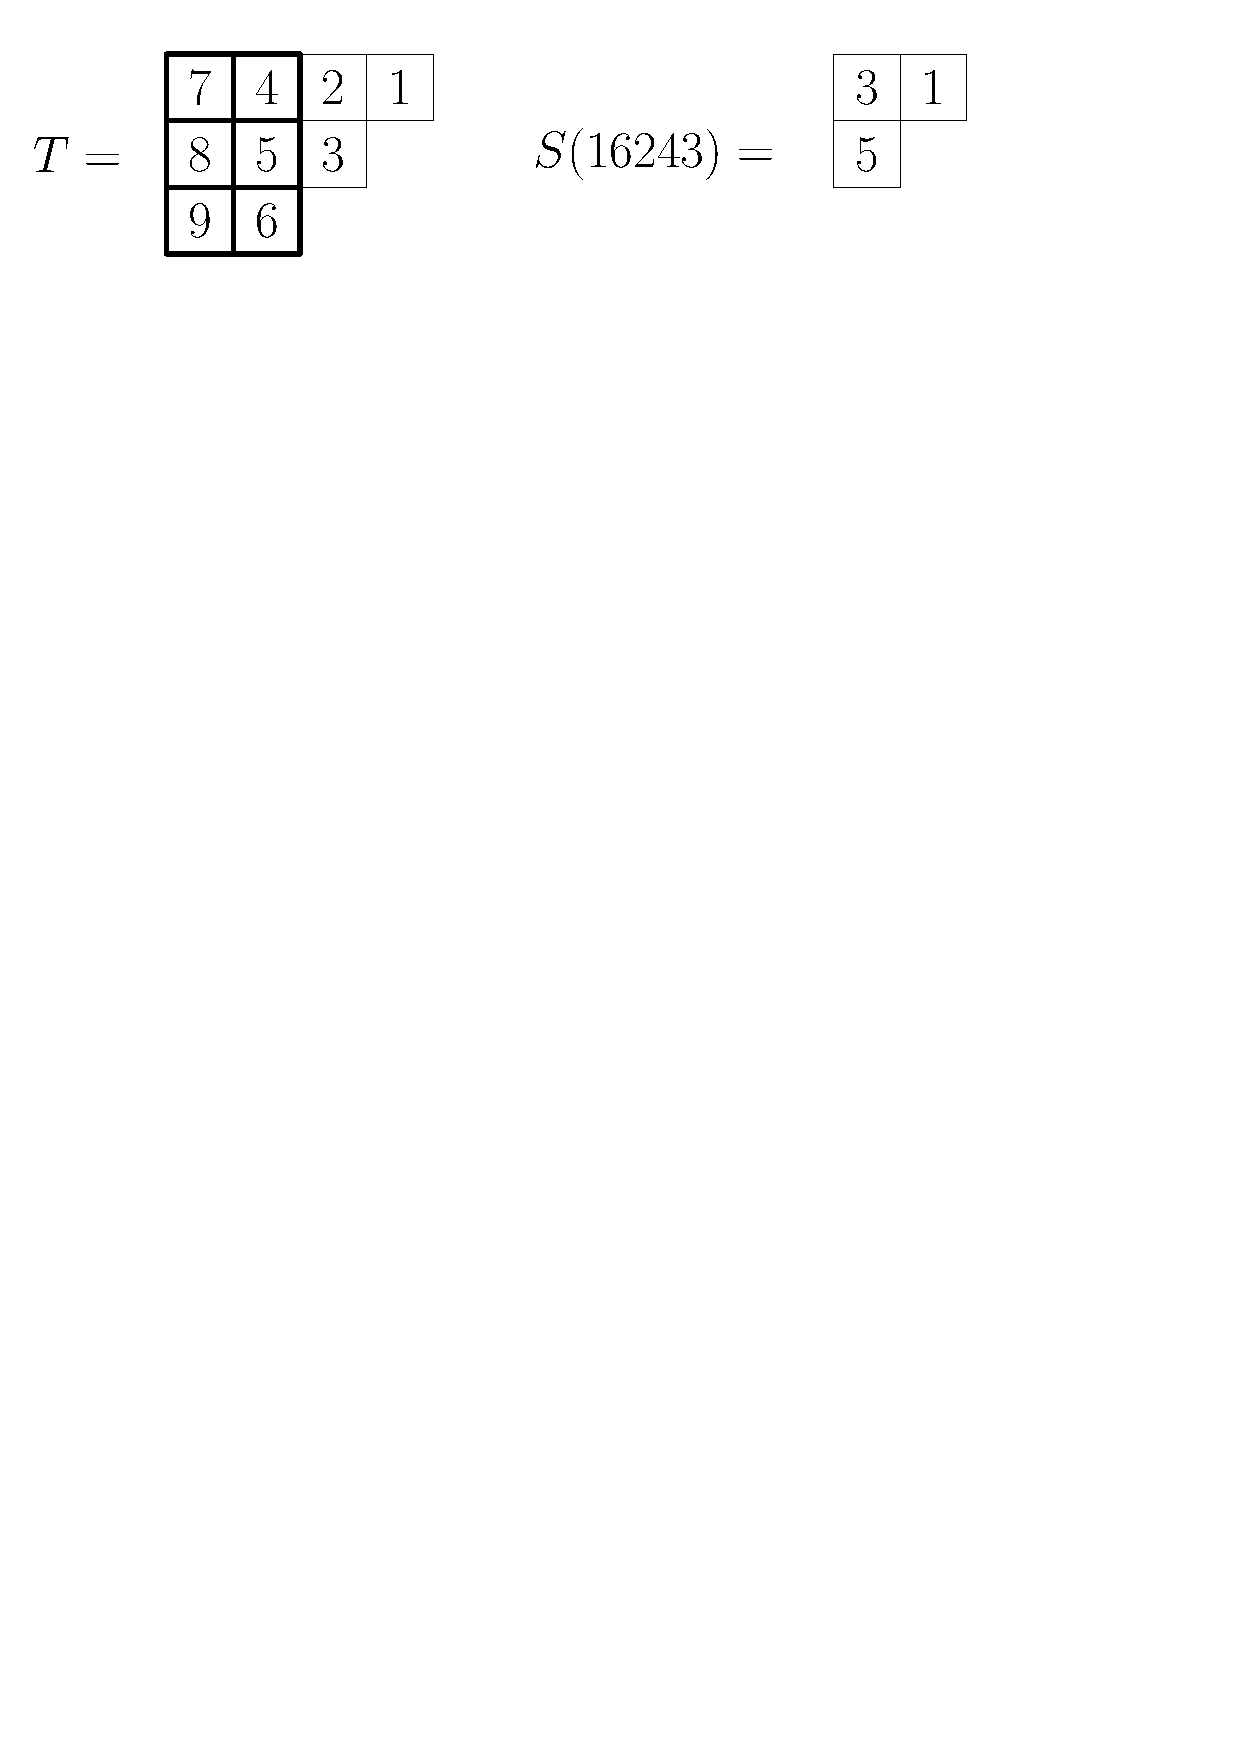
\includegraphics[scale=0.6]{Figures/SOfw.pdf}
  \caption{An example of $S(w)$ when $T$ is as shown, where $n=5$, $\la=(2,1)$, $s=3$, and $w=16243$.\label{fig:SOfw}} 
\end{figure}

\begin{lemma}\label{lem:IrredSubspaceUnion}
  For $S\in \mathcal{P}(n,\la)$, we have
  \begin{align}
    Y_{n,\la,s,T}^S = \bigsqcup_{\substack{w\text{ admissible},\\ S(w) \text{ column equivalent to }S}} C_w \cap Y_{n,\la,s,T}.
  \end{align}

  \begin{proof}
    For $w$ admissible, it can be checked by induction that the row-decreasing filling $S(w)$ is column equivalent to a unique element of $\mathcal{P}(n,\la)$. Since the cells $C_w\cap Y_{n,\la,s,T}$ partition $Y_{n,\la,s,T}$, it suffices to show the containment $C_w\cap Y_{n,\la,s,T}\subseteq Y_{n,\la,s,T}^S$ for the unique $S\in\mathcal{P}(n,\la)$ that is column equivalent to $S(w)$. Since $S$ and $S(w)$ are column equivalent, then $\sh(S|_{n-i+1,\dots, n}) = \sh(S(w)|_{n-i+1,\dots, n})$ for all $i\leq n$.

    Let $E_\bullet$ be the flag in $C_w\cap Y_{n,\la,s,T}$ defined by $E_i = \{f_{w(1)},\dots, f_{w(i)}\}$. It is easily checked that $N|_{F_k/E_i\cap F_k}$ has Jordan type $\sh(S(w)|_{n-i+1,\dots, n}) = \sh(S|_{n-i+1,\dots, n})$, so $E_\bullet\in Y_{n,\la,s,T}^S$. Let $i\leq s$ such that $w(1) = T(i,\Lambda_i)$. Recall from the proof of Lemma~\ref{lem:CellRecursion} that we have a map
    \[
      \Phi : \vspan\{f_{T(j,\Lambda_j)}\st j<i\}\times (C_{\fl_T^{(i)}(w)}\cap Y_{T^{(i)}}) \to C_w \cap Y_T.
      \]
      defined by
      \[
        \Phi(v,V_\bullet) = U_v(\langle f_{w(1)}\rangle, \langle f_{w(1)}\rangle + \psi^{(i)} (V_1),\dots, \langle f_{w(1)}\rangle + \psi^{(i)}(V_{n-1})).
      \]
      If $i>\ell(\la)$, then $N_T|_{F_k/(V_i\cap F_k)} = N_{T^{(i)}}|_{F_k/(V_{i-1}\cap F_k)}'$ and $S^{(i)} = S$, and we are done by induction.

      Otherwise, $i\leq\ell(\la)$, and we know by induction that for all $j$, $N_{T^{(i)}}|_{F_{k-1}/(V_j\cap F_{k-1})}$ has Jordan type $\sh(S^{(i)}|_{n-1,\dots, n-j})$. Now, we have
      \begin{align}
        N_T|_{F_k/(F_k\cap U_v(\langle f_{w(1)}\rangle + \psi^{(i)}(V_{j-1})))} = N_T |_{U_v(F_k/(F_k\cap (\langle f_{w(1)}\rangle + \psi^{(i)}(V_{j-1}))))}.
      \end{align}
      Since $U_v N_T = N_T U_v$, this map has the same Jordan type as $N_T|_{F_k/(F_k\cap (\langle f_{w(1)}\rangle + \psi^{(i)}(V_{j-1})))}$, which has the same Jordan type as $N_{T^{(i)}}|_{F_{k-1}/(F_{k-1}\cap V_{j-1})}$, which by our inductive hypothesis has Jordan type $\sh(S^{(i)}|_{n-j+1,\dots, n-1}) = \sh(S|_{n-j+1,\dots, n})$. Thus, the induction is complete.
    \end{proof}

    \begin{lemma}\label{lem:IrreducibleNonempty}
      Let $S\in \mathcal{P}(n,\la)$. Then the subspace $Y_T^S$ is nonempty if and only if either $s>\ell(\la)$, or $s=\ell(\la)$ and for all $i\leq n$ not in $S$ the labels of $S$ up to $i-1$ fill at least one row of $[\la]$.
    \end{lemma}

    \begin{proof}
            It can be checked that there exists an admissible $w$ that is column equivalent to $S$ if and only if the conditions in the statement of the lemma hold. Therefore, by Lemma~\ref{lem:IrredSubspaceUnion}, these are exactly the conditions for when $Y_T^S$ is nonempty.
    \end{proof}

    \begin{lemma}\label{lem:IrreducibleDimension}
      Let $S\in \mathcal{P}(n,\la)$. When $Y_T^S$ is nonempty, it is smooth and connected of dimension $n(\la) + (n-k)(s-1)$.
    \end{lemma}

    \begin{proof}
      Let $S\in \mathcal{P}(n,\la)$ that satisfies the conditions in the statement of Lemma~\ref{lem:IrreducibleNonempty}.  If $S$ contains the label $1$, let $(i,j)$ be the cell of $[\la]$ containing it. Otherwise, let $(i,j) = (s,n-k)$. It can be checked that $S^{(i)}$ satisfies the conditions in the statement of Lemma~\ref{lem:IrreducibleNonempty}, so $Y_{T^{(i)}}^{S^{(i)}}$ is nonempty. We have a surjective map $\pi$,
      \begin{align}
        Y_T^S \xrightarrow{\pi} \bP(\vspan\{f_{T(h,\Lambda_h)} \st h\leq i\}) \setminus \bP(\vspan\{f_{T(h,\Lambda_h)}\st h\leq \Lambda_{j+1}'\}).
      \end{align}
      defined by sending $V_\bullet$ to $V_1$. Let
      \begin{align}
        U \coloneqq \bP(\vspan\{f_{T(h,\Lambda_h)} \st h\leq i\}) \setminus \bP(\vspan\{f_{T(h,\Lambda_h)}\st h < i\}).
      \end{align}
      Assume by induction on $n$ that $Y_{T^{(i)}}^{S^{(i)}}$ are smooth and connected with dimension $n(\la^{(i)})+(n-k)(s-1)$ for $i\leq \ell(\la)$ and $n(\la)+(n-k-1)(s-1)$ for $i>\ell(\la)$.  Using Lemma~\ref{lem:IrredSubspaceUnion}, it can be checked that the isomorphisms $\Phi$ in the proof of Lemma~\ref{lem:CellRecursion} can be combined into an isomorphism
      \begin{align}
        U\times Y_{T^{(i)}}^{S^{(i)}} \to \pi^{-1}(U).
      \end{align}
     Thus, by the inductive hypothesis, the open subset $\pi^{-1}(U)$ of $Y_T^S$ is smooth and connected. Its dimension is
      \begin{align}
        \dim(U) + \dim(Y_{T^{(i)}}^{S^{(i)}}) &= (i-1) + \begin{cases} n(\la^{(i)}) + (n-k)(s-1) & i\leq \ell(\la)\\ n(\la) + (n-k-1)(s-1) & i>\ell(\la)\end{cases}\\
        &= n(\la) + (n-k)(s-1).
      \end{align}
      Given $\Lambda_{j+1}'+1\leq i' \leq i$, we have an open subset
      \begin{align}
        U_{i'} = \bP(\vspan\{f_{T(h,\Lambda_h)}\st h\leq i\})\setminus \bP(\vspan\{f_{T(h,\Lambda_h)}\st h\leq i, h\neq i'\})
      \end{align}
      of the codomain of $\pi$. By a similar construction as above, there is an isomorphism
      \begin{align}
        U_{i'}\times Y_{T^{(i)}}^{S^{(i)}}\to \pi^{-1}(U_{i'})
      \end{align}
      for each of these open subsets that cover $Y_T^S$, so $\pi^{-1}(U_{i'})$ is smooth of the same dimension. Since $Y_T^S$ is covered by smooth connected open subspaces of dimension $n(\la)+(n-k)(s-1)$, it follows that $Y_T^S$ is smooth of dimension $n(\la)+(n-k)(s-1)$. Since each $\pi^{-1}(U_{i'})$ is connected, and the intersection of these subspaces is nonempty intersection, then $Y_T^S$ is connected. The base case $n=1$ of the induction is trivial to check, so the proof is complete.
    \end{proof}

\end{lemma}



\begin{theorem}
The space $Y_{n,\la,s,T}$ is equidimensional of dimension $n(\la) + (n-k)(s-1)$. In particular, the closed subvarieties $\overline{Y_{n,\la,s,T}^{S}}$ for which $Y_{n,\la,s,T}^{S}$ is nonempty (as described in~Lemma \ref{lem:IrreducibleNonempty}) form a complete set of irreducible components. In the case $s>\ell(\la)$, there are $\binom{n}{k}\cdot \#\SYT(\la)$ many irreducible components.
\end{theorem}

\begin{proof}
By Lemma~\ref{lem:IrreducibleDimension}, the nonempty subspaces $Y_{n,\la,s,T}^S$ are smooth and connected of dimension $n(\la)+(n-k)(s-1)$. Therefore, $Y_{n,\la,s,T}^S$ is irreducible. Since the subspaces $Y_{n,\la,s,T}^S$ partition the space $Y_{n,\la,s,T}$, their closures form a complete set of irreducible components. When $s>\ell(\la)$, the irreducible components are thus in bijection with $\mathcal{P}(n,\la)$, which has cardinality $\binom{n}{k}\cdot \#\SYT(\la)$. This can be seen explicitly by relabeling $S$ by replacing each label $i$ with $n-i+1$ to get a row and column increasing tableau on $[\lambda]$ whose labels are chosen from a $k$-element subset of $[n]$.
\end{proof}



In the case $s>\ell(\la)$, the irreducible components are naturally indexed by Standard Young Tableaux on $\la \cup (n-k)$.  This indexing of irreducible components extends to a representation theory statement on the top cohomology group of $Y_{n,\lambda,s}$, generalizing Springer's theorem that the top cohomology group of a Springer fiber is a Specht module.
 

\begin{theorem}\label{thm:GenSpringerCorrespondence}
Let $d = \dim(Y_{n,\la,s}) = n(\la) + (n-k)(s-1)$, and consider $S_k$ as the subgroup of $S_n$ permuting the elements of $[k]$. For $s>\ell(\la)$, we have an isomorphism of $S_n$-modules
\begin{align}
H^{2d}(Y_{n,\la,s};\bQ) \cong \mathrm{Ind}\!\uparrow_{S_k}^{S_n} (S^\la).
\end{align}
For $s=\ell(\la)$, we have
\begin{align}\label{eq:SLengthLambdaIso}
    H^{2d}(Y_{n,\la,s};\bQ) \cong S^{\Lambda/(n-k)^{s-1}},
\end{align}
the Specht module of skew shape $\Lambda/(n-k)^{s-1}$.
\end{theorem}

Before we give the proof of this theorem, we recall a formula for the graded Frobenius characteristic of $R_{n,\la,s}$ proved in~\cite{GriffinOSP}. Define a \emph{partial row-decreasing filling} $\varphi$ of $[\Lambda]$ to be a filling of a subset of the cells of $[\Lambda]$ with positive integers (allowing repeated labels) such that the labels in each row are right justified and weakly decrease from left to right, and so that all cell of $[\la]$ are filled. Let $\mathrm{PRD}_{n,\la,s}$ be the set of partial row-decreasing fillings of $[\Lambda(n,\la,s)]$ with a total of $n$ filled cells. For $\varphi\in \mathrm{PRD}_{n,\la,s}$ and $(i,j)\in [\Lambda]$ a filled cell, let $\varphi_{i,j}$ be the label of $\varphi$ in that cell. Given a weak composition $\alpha$, we say that $\varphi$ is \emph{of type $\alpha$} if for each $i$, the letter $i$ appears $\alpha_i$ many times as a label in $\varphi$.

Given $\varphi\in \mathrm{PRD}_{n,\la,s}$, an \emph{inversion} of $\varphi$ is one of the following,
\begin{enumerate}
\item  [(I1)] A pair of cells $(i,j),(i',j)\in [\la]$ such that $i<i'$ and $\varphi_{i,j} > \varphi_{i',j}$,
\item  [(I2)] A pair of cells $(i,j),(i',j-1)\in [\la]$ such that $i'<i$ and $\varphi_{i,j} > \varphi_{i',j-1}$,
\item  [(I3)] A cell $(i,n-k+1)\in [\la]$ in the first column of $[\la]$ together with a filled cell $(i',j')\in [\Lambda]\setminus [\la]$ such that $i' < i$ and $\varphi_{i,n-k+1} > \varphi_{i',j'}$,
\item  [(I4)] A pair $(i,(i',j'))$ where $(i',j')$ is a filled cell of $[\Lambda]\setminus [\la]$ and $1\leq i<i'$.
\end{enumerate}
Let $\inv(\varphi)$ be the number of inversions of $\varphi$. \SG{For example...see Figure...}

\begin{remark}
The partial row-decreasing fillings defined here are a simple variation of the extended column-increasing fillings defined in~\cite{GriffinOSP}. There is an obvious bijection between $\mathrm{PRD}_{n,\la,s}$ defined here and $\mathrm{ECI}_{n,\la,s}$ defined in~\cite{GriffinOSP}: Given $\varphi\in \mathrm{PRD}_{n,\la,s}$, rotate the filling by 90 degrees counterclockwise, and delete all unfilled cells. The inversion statistics $\mathrm{inv}$ defined here is also a simple variation of the $\mathrm{inv}$ statistic in \cite{GriffinOSP}, which in turn is a variation on the \emph{coinversion} statistic on ordered set partitions originally defined by Rhoades, Yu, and Zhao in~\cite{Rhoades-Yu-Zhao}.
\end{remark}

We have the following formula for the graded Frobenius characteristic of $R_{n,\la,s}$. We state it in terms of partial row-decreasing fillings and powers of $q^2$ (due to our convention that $x_i$ has degree $2$).
\begin{theorem}[{\cite[Theorem 5.13]{GriffinOSP}}]\label{thm:grFrobTheorem}
  We have
  \[
    \Frob(R_{n,\la,s}^\bQ;q) = \sum_{\varphi \in \mathrm{PRD}_{n,\la,s}} q^{2\,\inv(\varphi)}\bx^\varphi,
  \]
  where $\bx^\varphi$ is the monomial such that the power of $x_i$ is the number of times $i$ appears as a label in $\varphi$.
\end{theorem}


\begin{proof}[Proof of Theorem~\ref{thm:GenSpringerCorrespondence}]
  By Theorem~\ref{thm:MainTheorem}, we have $H^*(Y_{n,\la,s};\bQ) \cong R_{n,\la,s}^\bQ$ as graded $S_n$-modules.
The case when $s>\ell(\lambda)$ follows immediately by combining this isomorphism with \cite[Corollary 3.3.15]{GriffinThesis}, which says that the top degree component of $R_{n,\lambda,s}$ is isomorphic as an $S_n$-module to $\mathrm{Ind}\!\uparrow_{S_k}^{S_n}\!(S^\lambda)$.

Let us now assume $s=\ell(\lambda)$. Combining Theorem~\ref{thm:MainTheorem} and Theorem~\ref{thm:grFrobTheorem}, we have that
\begin{align}\label{eq:FrobCohMonomial}
    \Frob(H^{2d}(Y_{n,\lambda,s};\bQ);q) = \sum_{\substack{\varphi \in \mathrm{PRD}_{n,\lambda,s},\\ \mathrm{inv}(\varphi)=d}} \mathbf{x}^\varphi.
\end{align}
It can be checked that $\inv(\varphi) = d$  if and only if the labels of $\varphi$ strictly decrease down each column and all filled cells of $[\Lambda]\setminus [\la]$ are in row $\ell(\lambda)$.

It suffices to prove that the right-hand side of \eqref{eq:FrobCohMonomial} is equal to the skew Schur function $s_{\Lambda/(n-k)^{\ell(\la)-1}}(\bx)$. Let $\alpha = (\alpha_1,\dots, \alpha_n)$ be a weak composition of $n$ into $n$ parts.
The $\bx^\alpha$ coefficient of the right-hand side of \eqref{eq:FrobCohMonomial} is the number of $\varphi\in \mathrm{PRD}_{n,\la,s}$ such that label $i$ appears $\alpha_i$ many times for each $i$ and $\mathrm{inv}(\varphi) = d$. 

Given $\varphi\in \mathrm{PRD}_{n,\la,s}$ of type $\alpha$ such that $\mathrm{inv}(\varphi) = d$, define a labeling $T$ of the Young diagram of skew shape $\Lambda/(n-k)^{\ell(\lambda)-1}$ by deleting all empty cells of $[\Lambda]$ and replacing each label $j$ with $n+1-j$. Since the labels of $\varphi$ weakly decreases from left to right along each row  strictly decrease down each column, then the labels of $T$ weakly increase left to right along each row and strictly increase down each column. Therefore, $T$ is a semi-standard Young tableau of type $(\alpha_n,\alpha_{n-1},\dots, \alpha_1)$. Moreover, $\varphi$ can easily be reconstructed from $T$. 

Therefore, the coefficient of $\bx^\alpha$ in the right-hand side of \eqref{eq:FrobCohMonomial} is equal to the coefficient of $\bx^{(\alpha_n,\alpha_{n-1},\dots, \alpha_1)}$ in $s_{\Lambda/(n-k)^{\ell(\la)-1}}(\bx)$. Since both $s_{\Lambda/(n-k)^{\ell(\la)-1}}(\bx)$ and the right-hand side of \eqref{eq:FrobCohMonomial} are symmetric, we conclude that these two symmetric functions are equal. Since $s_{\Lambda/(n-k)^{\ell(\la)-1}}(\bx)$ is the Frobenius characteristic of the skew Specht module $S^{\Lambda/(n-k)^{\ell(\la)-1}}$, the isomorphism~\eqref{eq:SLengthLambdaIso} holds, and the proof is complete.
\end{proof}

%In the case of $s>\ell(\la)$, the proof follows by combining Theorem~\ref{thm:MainTheorem} and the fact that, in this case, the top degree component of $R_{n,\lambda,s}$ is isomorphic to $\mathrm{Ind}\!\!\uparrow_{S_k}^{S_n}(S^\lambda)$~\cite[Corollary 3.3.15]{GriffinThesis}. In the case of $s=\ell(\la)$, the proof follows by combining Theorem~\ref{thm:MainTheorem} with the formula \cite[Theorem 5.13]{GriffinOSP} for $\Frob(R_{n,\lambda,s};q)$ and then using bijective techniques to show that the top degree component of this symmetric function is the skew Schur function $s_{\Lambda/(n-k)^{s-1}}(x)$.




%%%%%%%%%%%%%%%%%%%%%%%%%%%%
\section{The space $Y_{n,\lambda}$}\label{sec:IndVariety}
%%%%%%%%%%%%%%%%%%%%%%%%%%%%

In this section, we construct a topological space $Y_{n,\lambda}$ whose cohomology ring is isomorphic to $R_{n,\lambda}$. We then state a generalization of a theorem of de Concini and Procesi that relates Springer fibers to the scheme of diagonal ``nilpotent'' matrices.



For any $n$ and $\lambda\vdash k$, define the topological space $Y_{n,\la}$ as follows. Let $N$ be a nilpotent operator on the $\bC$-vector space $\bC^\infty$ with countably infinite dimension that has Jordan type \[(n-k+\la_1, \dots, n-k+\la_{\ell(\la)}, n-k,n-k,\dots).\] 
Then $\im(N^{n-k})$ has dimension $k$. We define the following topological space,
\begin{align}
    Y_{n,\la}\coloneqq \{V_\bullet\in \Fl_{(1^n)}(\bC^\infty)\st NV_i\subseteq V_i \text{ for }i\leq n\text{ and }\im(N^{n-k})\subseteq V_n\}.
\end{align}
We have closed embeddings
\[
Y_{n,\la,\ell(\la)}\subseteq Y_{n,\la,\ell(\la)+1}\subseteq\cdots\subseteq Y_{n,\la,s}\subseteq\cdots.
\]
It can be checked that $Y_{n,\la}$ is the direct limit of these topological spaces,
\[Y_{n,\la} \cong \varinjlim_s Y_{n,\la,s}.\]

%Let us recall the Universal Coefficient Theorem for Cohomology. It states that given any space $X$, there exists a split exact sequence
%\[
%0\to \mathrm{Ext}^1_\bZ(H_{i-1}(X),\bZ)\to H^i(X)\stackrel{h}{\to} \Hom(H_i(X),\bZ)\to 0
%\]
%where the map $h$ is defined as follows: given $\varphi: C_i(X)\to \bZ$ an $i$-cocycle, then $\delta \varphi =0$, where $\delta$ is the differential map on singular cocycles. Therefore,  we have $\varphi|_{B_i(X)}=0$, so %$\varphi$ induces a map $\overline \varphi :Z_i(X)/B_i(X)\to \bZ$. The map $h$ is defined by $h([\varphi]) \coloneqq \overline\varphi$.


\begin{theorem}
We have $H^*(Y_{n,\la})\cong R_{n,\la}$ as graded rings.
\end{theorem}

\begin{proof}
By Theorem~\ref{thm:MainTheorem}, we have $H^*(Y_{n,\lambda,s})\cong R_{n,\la,s}$ From the definitions of $R_{n,\la}$ and $R_{n,\la,s}$, it can be checked that
\begin{align}
R_{n,\la} \cong \varprojlim_s H^*(Y_{n,\la,s}),
\end{align}
where the inverse limit is taken in the category of graded rings. Since each $Y_{n,\la,s}$ is a complex variety with an affine paving, we have
\begin{align}
  \varprojlim_S H^*(Y_{n,\la,s}) \cong H^*(\varinjlim_s Y_{n,\la,s}) = H^*(Y_{n,\la}),
\end{align}
see e.g.~\cite[Lemma 7.2]{Pawlowski-Rhoades}, which completes the proof.
\end{proof}





%%%%%%%%%%%%%%%%%%%%%%%%%%%%
\section{Future Work}\label{sec:FutureWork}
%%%%%%%%%%%%%%%%%%%%%%%%%%%%

\begin{question}
Springer fibers have a natural type-independent description to other Lie types. Can the varieties $Y_{n,\la,s}$ be generalized to this setting, or for classical types?
\end{question}

\begin{question}
  The variety $Y_{n,\la,s}$ is simulaneously the projective image of a Spaltenstein variety and a closed subvariety of a Steinberg variety,
  \[
\cB_{(1^n,s-1,\dots,s-1)}^\Lambda \twoheadrightarrow Y_{n,\la,s}\hookrightarrow \{V_\bullet\in \Fl_{(1^n,(n-k)(s-1))}(\bC^K) \st N_\Lambda V_i\subseteq V_i \text{ for all }i\}.
\]
The Steinberg varieties are fibers of partial resolutions of the nilpotent cone~\cite{Goresky-Macpherson}, and Spaltenstein varieties have connections to representations of the general linear groups~\cite{Braverman-Gaitsgory}, crystals~\cite{Malik} and quiver varieties~\cite{Nakajima1,Nakajima2}. Do the varieties $Y_{n,\la,s}$ have any applications to these settings?
\end{question}

%\begin{question}
%There is a $s$-dimensional torus action on $Y_{n,\la,s}$, given by scaling the vectors in each generalized eigenspace of $N$ by the same constant. The space $Y_{2,\emptyset,2}$ is not a GKM variety because it does not have finitely many one-dimensional orbits with respect to this action. Is it still possible to compute its equivariant cohomology ring? Brundan and Ostrik reference Goresky-Macpherson's characterization of equiv cohomology of Springer fibers in terms of subspace arrangements, and extensions of those results.
%\end{question}

\begin{question}
What are the cell closures for the paving of $Y_{n,(1^k),k}$? Is there a nice description of the corresponding ``Bruhat poset''?
\end{question}

%\begin{question}
%Can we identify the cohomology classes of the cell closures in the case of $Y_{n,(1^k),k}$?
%\end{question}

 
 
 \begin{question}
 The space $Y_{n,\la,s}$ in general singular because it has many irreducible components. Under what condition are all of the irreducible components smooth? Is this true for $Y_{n,(1^k),k}$, in particular?
\end{question}




\section{Acknowledgements}

We are grateful to Sara Billey, Erik Insko, Isabella Novik, Julia Pevtsova, Martha Precup, Brendon Rhoades, and Andy Wilson for helpful conversations.


\bibliographystyle{hsiam}
\bibliography{Springer}

\end{document}



